%!TEX root = ../../thesis.tex
\chapter[Available energy of trapped electrons]{Available energy of trapped electrons}
\label{chap: AE-TE}
With our understanding of the bounce-averaged drift cemented, we now shift our focus to the \AE{} of trapped electrons. Let us note that this publication has been published in two parts. Firstly, a highly condensed version of the results presented was published as a {\it Physical Review Letter} for a general physics audience \cite{mackenbach2022available}. In a later publication, we included additional findings in the research and gave more details of the derivation, and this publication is what we include in the thesis. The publication focusses on the \AE{} of trapped electrons, as eluded to before, where the result of \cite{helander2020available} will be generalised to account for radially drifting trapped particles. The generalised expression of the \AE{} of trapped electrons allows us to compare it with nonlinear gyrokinetics in general magnetic geometries. Before the research, it was unknown whether \AE{} of trapped electrons can be used to predict turbulent transport, and in the following research we find predictive capabilities. This finding is encouraging, as it implies that \AE{} can be used as a measure of turbulent transport in general systems, making it useful in, e.g., optimisation loops. \vfill \newpage

\section*{The available energy of trapped electrons: a nonlinear measure for turbulent transport}
\small{R.J.J. Mackenbach$^{1,2}$, J.H.E. Proll$^{1,2}$, R. Wakelkamp$^{3}$ P. Helander$^{2}$} \\
\small{$^1$ Eindhoven University of Technology, 5612 AZ, Eindhoven, Netherlands} \\
\small{$^2$ Max Planck Institute for Plasma Physics, 17491 Greifswald, Germany} \\
\small{$^3$ Utrecht University, 3584 CS Utrecht, The Netherlands}


\chapterabstract{A collisionless plasma possesses a certain amount of ``available energy'', which is that part of the thermal energy that can be converted into kinetic energy of plasma motion and electromagnetic fluctuations. In this paper we present a calculation of the available energy carried by trapped electrons in a slender non-omnigenous flux tube of plasma. This quantity is compared with gyrokinetic simulations of the nonlinear saturated radial energy flux resulting from turbulence driven by collisionless trapped-electron modes in various stellarators and a tokamak. The numerical calculation of available energy is fast and shows a strong correlation with the turbulent energy fluxes found in the gyrokinetic simulations. Indeed, the energy flux is found to be proportional to the available energy to the power of approximately $3/2$, which is what one would expect from a simple argument. We furthermore investigate how available energy is distributed across different bounce wells, and it is found that deeply trapped electrons typically contribute most to the available energy. Finally, we investigate the dependence of available energy on gradient strength, and we find important differences between weakly and strongly driven regimes for stellarators and tokamaks.}

\section{Introduction} \label{sec:outline}
    One of the major challenges facing magnetically confined fusion plasmas is the degradation of energy confinement due to transport. This transport arises because the density and temperature vary across the plasma volume, giving rise to neoclassical transport as well as free energy which drives instabilities, turbulence, and transport. The dependence on the geometry of the magnetic field is well understood in the case of neoclassical transport, and stellarators can be designed in such a way as to minimize these losses \citep{Wolf2017MajorStellarator,Klinger2019OverviewOperation,Dinklage2018MagneticStellarator,beidler2021demonstration}. \par
    The main transport channel is then turbulent transport, which typically exceeds the neoclassical channel, see e.g. \citet{Bozhenkov2020High-performance7-X,beidler2021demonstration}. Accordingly, insights into the interplay between turbulence and geometry are desired so that one can understand, and perhaps minimize, the turbulent losses. However, due to the complex nonlinear nature of the problem, it has proved difficult to quantify the dependence of turbulence on geometry, though significant strides have been made in recent years \citep{Barnes2011CriticallyPlasmas,Proll2012ResilienceInstabilities,Proll2022TurbulenceGradient,Pueschel2016StellaratorModeling,Citrin2017TractableQuaLiKiz,Helander2013CollisionlessModes,Plunk2014CollisionlessMode}. 
    These methods, though not all of them, typically employ (quasi-)linear theory to estimate the turbulence properties for any given configuration. Such methods do not always capture important nonlinear effects and suffer, in particular, from uncertainties concerning the turbulent saturation amplitude. The most reliable option to assess nonlinear turbulent transport is to carry out nonlinear gyrokinetic simulations \citep{Beer1995FieldTurbulence,Garbet2010GyrokineticTransport}, but it is currently computationally expensive to do so, though significant improvements have been made \citep{Mandell2022GX:Design}. \par
    In a recent publication \citep{Mackenbach2022AvailableTransport}, it was shown that the so-called available energy (\AE{}) can provide a quantitative estimate of the turbulence driven by the trapped-electron mode \citep{Kadomtsev1967PlasmaGeometry,Dannert2005GyrokineticTurbulence}, and in the present paper we elaborate on the mathematical details of this calculation. 
    \par
    The \AE{} of a system is defined as the difference in energy between the ``initial'' distribution function $f_i$ (i.e. the distribution function at time $t=0$), and the so-called ground state $f_g$ \citep{Lorenz1955AvailableCirculation,Gardner1963BoundPlasma}. The latter is the distribution function which minimizes the energy, subject to constraints imposed by the Vlasov equation. We encapsulate the constraints that follow from Liouville's theorem in the following invariant
    \begin{equation}
    H[f(\boldsymbol{x},t),\phi] \equiv \int \Theta[f(\boldsymbol{x},t)-\phi] \mathrm{d} \boldsymbol{x},
    \label{eq:vlasov-invariant}
    \end{equation}
    where $\Theta[x]$ is the Heaviside function, $\phi$ is a scalar constant, and $\boldsymbol{x}$ are the phase-space coordinates, $(\boldsymbol{r},\boldsymbol{v})$. If the distribution function $f$ evolves according to the Vlasov equation or any other equation that conserves phase-space volume, one can show that $H[f,\phi]$ is conserved for every $\phi \in \mathbb{R}$ \citep{Helander2017AvailablePlasmas}. Furthermore, we define the energy of the distribution function as
    \begin{equation}
        E[f(\boldsymbol{x},t)] \equiv \int \epsilon (\boldsymbol{x}) f(\boldsymbol{x},t) \mathrm{d} \boldsymbol{x},
    \label{eq:energy-functional}
    \end{equation}
    where $\epsilon(\boldsymbol{x})$ is the energy of a particle (typically $mv^2/2$). With these definitions, the ground state can be denoted as the distribution function t minimizes the functional
    \begin{equation}
        W[f_g,\lambda] = E[f_g] + \int \lambda(\phi) \left( H[f_i,\phi] - H[f_g,\phi] \right) \mathrm{d}\phi
    \end{equation}
    where $\lambda(\phi)$ denotes a continuous set of Lagrange multipliers. \par
    If one evaluates the variation of $W$ with respect to $f_g$, and requires that the distribution function be a stationary point of the functional (that is $\delta W/\delta f_g=0$), one finds that a ground state must be a function of energy alone,
    \begin{equation}
        f_g = f_g(\epsilon).
        \label{eq:ground-state-dependencies}
    \end{equation}
    Furthermore, if one considers the second variation with respect to $f_g$ and demands that this quantity be positive definite (so that the ground state is a local minimum of the functional), one finds that the ground state must be a decreasing function of energy
    \begin{equation}
        \frac{\partial f_g}{\partial \epsilon} \leq 0.
        \label{eq:ground-state-energy-dependence}
    \end{equation}
    \par
    One can also impose the condition that a set of adiabatic invariants, denoted by $\boldsymbol{y}$, should be conserved (as in \cite{Helander2017AvailablePlasmas,Helander2020AvailablePlasmas}), thus adding more constraints than equations \eqref{eq:ground-state-dependencies} and \eqref{eq:ground-state-energy-dependence}. The ground states are then functions satisfying
    \begin{subequations}
    \begin{equation}
        f_g = f_g(\epsilon, \boldsymbol{y}),
    \end{equation}
    \begin{equation}
        \left( \frac{\partial f_g}{ \partial \epsilon } \right)_{\boldsymbol{y}}  \leq 0.
    \end{equation}
        \label{eq:ground-state-decrease-adiabatic}
    \end{subequations}
    \par 
    From these criteria it is possible to derive an integro-differential equation for the ground state. For instance, it has been shown that, if we choose the magnetic moment $\mu$ and the parallel invariant $\mathcal{J}$ as adiabatic invariants, the ground state $f_g(\epsilon,\mu,\mathcal{J})$ must obey the following integro-differential equation \citep{Helander2020AvailablePlasmas}
    \begin{equation}
    \begin{aligned}
        \left( \frac{ \partial f_g(w,\mu,\mathcal{J})}{\partial w} \right)_{\mu,\mathcal{J}} = - \frac{\iint \delta [w - \epsilon(\psi,\alpha,\mu,\mathcal{J})] \mathrm{d}\psi \mathrm{d}\alpha }{\iint \delta[f_i - f_g(w,\mu,\mathcal{J})] \mathrm{d}\psi \mathrm{d}\alpha }.
    \end{aligned}
    \label{eq:ground-state-eq}
    \end{equation}
    Here $w$ is a positive scalar which acts as a placeholder for the particle energy $\epsilon$, $\psi$ is the magnetic flux (i.e. the flux-surface label) and $\alpha$ is the Clebsch angle, which locally define the magnetic field as $\boldsymbol{B} = \nabla \psi \times \nabla \alpha $ \citep[see][ch.~5]{Dhaeseleer2012FluxTheory}. Equation \eqref{eq:ground-state-eq} is relevant for most kinds of gyrokinetic turbulence in tokamaks and stellarators, since $\mu$ and $\mathcal{J}$ are typically conserved quantities for trapped electrons in the case of microinstabilities and turbulence with wavelengths comparable to the ion gyroradius. 
    \par
    In the literature, most numerical simulations of such phenomena are performed in the geometry of a slender flux tube aligned with the magnetic field, and in this limit Eq.~(\ref{eq:ground-state-eq}) can be solved analytically. For the case of a vanishingly slender flux tube under the condition of omnigenity, i.e. that the second adiabatic invariant $\mathcal{J}$ is independent of the Clebsch angle $\alpha$ (i.e. $\partial \mathcal{J} / \partial \alpha = 0$), explicit expressions for the ground state and the \AE{} have been found \citep{Helander2020AvailablePlasmas}. This derivation shows that a Maxwellian distribution function can only be a ground state if the magnetic field is omnigenous and if the electron diamagnetic drift frequency $\omega_*^T$ does not exceed the bounce-averaged precession frequency $\omega_\alpha$,
    \begin{equation}
        \omega_*^T/\omega_\alpha \leq 1,
        \label{eq:stability-crit}
    \end{equation}
    for all types of trapped-electron orbits in the flux tube. Here the diamagnetic drift frequency is equal to
    \begin{equation}
        \omega_*^T = \frac{T}{q} \left[ \frac{\mathrm{d} \ln n}{\mathrm{d} \psi} + \frac{\mathrm{d} \ln T}{\mathrm{d} \psi} \left( \frac{\epsilon}{T} - \frac{3}{2} \right) \right],
    \end{equation}
    where $T$ is the temperature, $n$ is the number density, $\epsilon$ is the particle energy, and $q$ is the particle charge.
    The criteria of \eqref{eq:stability-crit} are met in quasi-isodynamic stellarators with the so-called maximum-$\mathcal{J}$ property, and it has been shown from the (linear) gyrokinetic equations that these devices are indeed resilient against conventional density-gradient-driven TEMs by \citep{Proll2012ResilienceInstabilities,Helander2013CollisionlessModes}. When these modes are stabilised, other, less virulent, instabilities become dominant instead \citep{Helander2015TheGeometry,Plunk2017CollisionlessMode,costello2023universal}.
    \par 
    In this paper we first extend the calculation of \AE{} to non-omnigenous flux-tubes, which is of relevance since most stellarators are, in fact, not omnigenous. We first show that such a calculation is most easily done in flux tubes which have an elliptical cross-section. This calculation is described in section \ref{sec:theory}, where we also discuss how the \AE{} can be computed numerically. In section \ref{sec:results} we compare the numerically calculated \AE{} in a tokamak and various stellarators with the turbulent energy flux computed by the gyrokinetic code \textsc{gene} \citep{Jenko2000ElectronTurbulence}. These results were recently published in abbreviated form \citep{Mackenbach2022AvailableTransport}, and here we provide full mathematical details. We furthermore investigate which types of trapped particles contribute most to \AE{}, and find that deeply trapped particles typically do so. We also establish that the dependence on the gradient strength is non-trivial and investigate this dependence in some depth. Finally, in section \ref{sec:conclusions}, we highlight our most important findings and discuss future directions for research. 
 
\section{The ground state and available energy in a flux-tube} \label{sec:theory}
\subsection{Allowable domains}
In the calculation of the ground state, we restrict our attention to a subregion of the plasma which has the shape of a slender flux tube aligned with the magnetic field, allowing us to approximate the distribution function by its first-order Taylor expansion in the directions perpendicular to the field. Only then does it seem possible to solve the integro-differential ground-state equation (\ref{eq:ground-state-eq}) in general. Somewhat surprisingly, it turns out that the calculation is only possible if the cross section of the flux tube is elliptical, as we shall now see. 

We first introduce the following re-scaled coordinates,
\begin{subeqnarray}
    x &&= (\psi - \psi_0)/\Delta \psi, \\
        y &&= (\alpha - \alpha_0)/\Delta \alpha.
        \label{eq:altered-coordinates}
\end{subeqnarray}
Here, $\psi_0$ and $\alpha_0$ are the flux-surface label and field-line label of the magnetic field line defining the centre of the flux tube, and $\Delta \psi$ and $\Delta \alpha$ define its scale lengths in the $\psi$- and $\alpha$-directions, respectively. In contrast to the situation in most gyrokinetic simulations, the cross section of the flux tube is not assumed to be rectangular. In these coordinates, we denote the first-order expansion of the distribution function $f$ for fixed values of $\mu$, $\mathcal{J}$, and $t$ by
\begin{equation}
        f(x,y,\mu,\mathcal{J},t) \equiv f_0 + f_{x} x + f_{y} y.
        \label{eq:expansion}
\end{equation}
For a given smooth distribution function, this representation should always be sufficiently accurate in the limit of small $\Delta \psi$ and $\Delta \alpha$ (i.e. for small enough $\psi - \psi_0$ and $\alpha - \alpha_0$ one can approximate $f \approx f_0 + (\psi - \psi_0) \partial_\psi f + (\alpha - \alpha_0) \partial_\alpha f$), but there is no guarantee that the ground state corresponding to such a function can be similarly approximated by its linear expansion. Indeed, this turns out to be true, in general, only if the domain $\Omega$ in the $(x,y)$-plane under consideration is elliptical. 
As already mentioned, phase-space volume conservation dictates that the following integral is independent of time for all values of $\phi$,
\begin{equation}
    \frac{\mathrm{d}}{\mathrm{d} t}\int_{\Omega} \Theta \left[ \phi - f(x,y,\mu,\mathcal{J},t) \right] \mathrm{d} x \mathrm{d} y = 0.
    \label{eq:vlasov-inv}
\end{equation}
In particular, this integral must be the same for the initial (given) distribution function and its corresponding ground state. We assume that both can be described by their linear approximations (\ref{eq:expansion}), whose gradients will, however, in general point in different directions (i.e. $\nabla_\perp f \propto \hat{\boldsymbol{x}} f_x +\hat{\boldsymbol{y}} f_y$ can take on any value, with the hatted quantities denoting unit vectors). We thus require that the gradient of the ground state may point in an arbitrary direction and derive a constraint on the shape of $\Omega$ from this condition.

It is useful to define a rotated coordinate system $(x,y)\mapsto(\tilde{x},\tilde{y})$, 
\begin{equation}
\begin{aligned}
\tilde{x} &= x \cos \vartheta + y \sin \vartheta + x_{\rm min}(\vartheta), \\
\tilde{y} &= - x \sin \vartheta + y \cos \vartheta + y_{\rm min}(\vartheta),
\end{aligned}
\end{equation}
such that $f$ assumes its smallest value, $f_{\rm min}$, at $\tilde x = 0$ and the gradient of $f$ points in the direction of $\tilde x$:
\begin{equation}
    f = f_\mathrm{min} + f_{\tilde{x}} \tilde{x}.
\end{equation}
In such a coordinate system the domain rotates as the function evolves, whilst fixing the minimal values of $x$ and $y$ to $\tilde{x}=\tilde{y}=0$, and this coordinate system will aid us in making statements about this domain shape. The initial state and the ground state thus correspond to two different values of $\vartheta$. The width of the domain $\Omega$ in the $\tilde x$-direction is denoted by $2D(\vartheta)$, so that the maximum value of $f$ becomes $f_\mathrm{max} = f_\mathrm{min} + 2 D f_{\tilde{x}}$, and the distribution function may be written as
\begin{equation}
    f = f_\mathrm{min} + \frac{\tilde{x}}{2D} \left( f_\mathrm{max} - f_\mathrm{min} \right),
\end{equation}
where we note that $f_\mathrm{min}$ and $f_\mathrm{max}$ depend only on $\mu$ and $\mathcal{J}$ and are thus independent of $\vartheta$. 

We now return to the problem at hand, codified by Eq. \eqref{eq:vlasov-inv}. The argument of the Heaviside function vanishes in the new coordinate system when
\begin{equation}
    \tilde{x}(\phi) = 2D \frac{\phi - f_\mathrm{min}}{f_\mathrm{max}-f_\mathrm{min}}.
        \label{eq:zero-of-heaviside}
\end{equation}
Let us now consider a value of $\phi$ very close to $f_\mathrm{min}$, i.e. $\phi = f_\mathrm{min} + |\epsilon|$ with $|\epsilon| \rightarrow 0^+$. Eq. \eqref{eq:zero-of-heaviside} now reduces to $\tilde{x}_\epsilon = 2D|\epsilon|/(f_\mathrm{max}-f_\mathrm{min})$. The integral in Eq.~(\ref{eq:vlasov-inv}) is equal to the area of the subdomain of $\Omega$ over which $f \le \phi$, i.e. the coloured region in Fig. \ref{fig:sketch-of-area}. In the limit $\tilde{x}_\epsilon \ll D$, the radius of curvature, $R$, of the domain boundary in the region $\tilde x < \tilde x_\epsilon$ is approximately constant (if the boundary is sufficiently smooth). Hence, we may approximate the integral by instead considering the area of a circular segment with the same radius of curvature $R$,
\begin{equation}
\begin{aligned}
    \mathcal{A} &= 2\int_0^{\tilde{x}_\epsilon} \sqrt{2R\tilde{x}  - \tilde{x}^2} \: \mathrm{d} \tilde{x}  \\
    &\approx 2 \int_0^{\tilde{x}_\epsilon} \sqrt{2 R\tilde{x} } \: \mathrm{d} \tilde{x} = \frac{4}{3} \sqrt{2 R \tilde{x}_\epsilon^3},
\end{aligned}
\label{eq:circular-segment}
\end{equation}
\begin{figure}
    \centering
    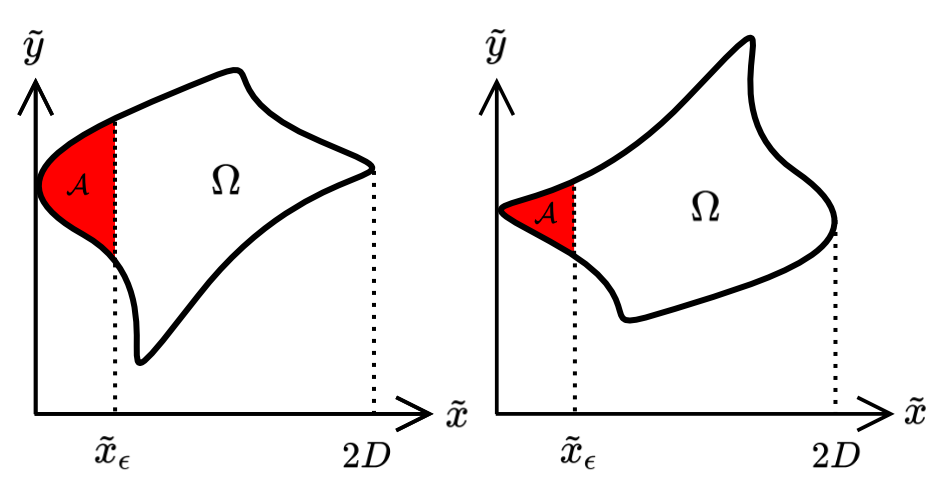
\includegraphics[width=1.0\textwidth]{3_chapters/1_papers/AE-TE/figures/boundary-setup.png}
    \caption{A sketch of the area, coloured red, as a subset of the entire domain $\Omega$. Done at two different times, so that the orientation of the domain $\Omega$ is different.}
    \label{fig:sketch-of-area}
\end{figure}
where we have used the equation for a circle $\tilde{y}^2 = R^2 - (\tilde{x} - R)^2 $. The next step is to realise that, as the distribution function evolves, its gradient may point in any direction in the $(x,y)$-plane, so that the angle $\vartheta$ may assume any value. A sketch of the domain at a different orientation is also given in Fig. \ref{fig:sketch-of-area}. Both $D$ and $R$ depend on $\vartheta$, but they are not independent. Indeed, from Eq. \eqref{eq:vlasov-inv}  we have
\begin{equation}
    R(\vartheta)D(\vartheta)^3 = C_\mathcal{A} = \mathrm{constant},
\end{equation}
where we have used the equation for the area found in \eqref{eq:circular-segment}. In particular, the radius of curvature is the same at the two extremal locations $\tilde{x}=0$ and $\tilde{x}=2D$, since a rotation of $\pi$ leaves $D$ unchanged. Moreover, on purely geometrical grounds there is a relation between the second derivative of the domain width and the curvature, as shown in Appendix \ref{app:diff-for-domain},
\begin{equation}
    \frac{\mathrm{d}^2 D}{\mathrm{d} \vartheta^2} = R - D.
\end{equation}
Using the constancy of $RD^3$, we find that
\begin{equation}
    \frac{\mathrm{d}^2 D}{\mathrm{d} \vartheta^2} + D = \frac{C_\mathcal{A}}{D^3} \implies \frac{\mathrm{d}}{\mathrm{d} \vartheta} \left[\left(\frac{\mathrm{d} D}{\mathrm{d} \vartheta}\right)^2 + D^2 + \frac{C_\mathcal{A}}{D^2} \right]=0.
\end{equation}
As shown in Appendix \ref{app:diff-for-domain}, this differential equation has the general solution
\begin{equation}
    D(\vartheta) = (C^2-C_\mathcal{A})^{1/4}\sqrt{C + \cos 2 \vartheta},
\end{equation}
implying that the radius of curvature becomes
\begin{equation}
    R(\vartheta) = \frac{C_\mathcal{A}}{(C^2-C_\mathcal{A})^{3/4}(C + \cos 2 \vartheta)^{3/2}}.
    \label{eq:radius-of-curvature-main}
\end{equation}
The radius of curvature for an ellipse is of the exact same form as Eq. \eqref{eq:radius-of-curvature-main} (as shown in the Appendix \ref{app:diff-for-domain}), implying that $\Omega$ must be elliptical. We have thus found that the only domain shape in which Liouville's theorem can generally be satisfied is a slanted ellipse, if the distribution function is to be approximated by its first-order Taylor expansion in the coordinates perpendicular to the magnetic field.

\subsection{The ground state and the available energy}
As shown in the previous section the domain has to be a slanted ellipse, and here we shall derive what the ground state and \AE{} is in such a system. To this end, let us first realize that it is sufficient to calculate the \AE{} in an {\it unslanted} ellipse, which in the coordinates $x$ and $y$ of the previous section has the equation
\begin{equation}
    \frac{x^2}{a^2} + \frac{y^2}{b^2} = 1,
    \label{eq: circle equation}
\end{equation}
with $a \leq b$. We may then apply a rotation-operator, to find the result of any slanted ellipse. Let us start, then, by considering equation \eqref{eq:ground-state-eq} and one must evaluate integrals of the form
\begin{equation}
    I[h] = \int_\Omega \delta[h] \mathrm{d}\psi \mathrm{d}\alpha,
    \label{eq:dirac-delta}
\end{equation}
where $h(\psi,\alpha)$ is an arbitrary smooth function that vanishes in the centre of the domain, $h(0,0)=0$. This condition has to do with the fact that a constant Maxwellian is the ground state corresponding to an initial condition without gradients. As such, to lowest order the difference between the Maxwellian and the ground state should vanish, implying that $h(0,0)=0$ for the functions appearing in \eqref{eq:ground-state-eq}. Since we take the flux tube to be slender, we approximate the function $h$ as
\begin{equation}
    h(\psi,\alpha) \approx x \Delta \psi \partial_\psi h + y \Delta \alpha \partial_\alpha h.
\end{equation} 
We next define the vector $\boldsymbol{p} = \left( x, y \right)$, so that one can write the linear expansion of $h$ as
\begin{equation}
    h \approx \boldsymbol{p} \cdot \boldsymbol{n} |\partial_{\boldsymbol{p}} h|,
\end{equation}
where we have defined $\boldsymbol{n} \equiv \partial_{\boldsymbol{p}} h/ |\partial_{\boldsymbol{p}} h| $, and derivatives of $h$ are evaluated at the centre of the flux tube. Equation \eqref{eq:dirac-delta} then becomes,
\begin{equation}
    I[h] = \frac{\Delta \psi \Delta \alpha }{|\partial_{\boldsymbol{p}} h|} \int_\Omega \delta[\boldsymbol{p} \cdot \boldsymbol{n}] \mathrm{d}x \mathrm{d}y.
\end{equation}
The integral measures the length of the line where $h=0$ in the domain, which may be found as follows. We realise that this line satisfies the equation
\begin{equation}
    y = -\frac{h_x}{h_y} x,
\end{equation}
where we have used the notation $h_x \equiv \partial_x h$. We may now find its intersection with Eq. \eqref{eq: circle equation}, and one may readily verify that the intersection satisfies the equation
\begin{equation}
    x^2 + y^2 = (ab)^2 \frac{(h_x)^2+( h_y)^2}{(a h_x)^2+(b h_y)^2},
\end{equation}
with which the integral becomes
\begin{equation}
\begin{aligned}
    I[h] &= \frac{\Delta \psi \Delta \alpha }{|\partial_{\boldsymbol{p}} h|}  2ab\sqrt{\frac{h_x^2 + h_y^2}{(a h_x)^2+(b h_y)^2}} \\
    &= \Delta \psi \Delta \alpha \frac{ 2 ab }{\sqrt{(ah_x)^2+(bh_y)^2}},
    \label{eq: unslanted ellipse ground state}
\end{aligned}
\end{equation}
Our final step is to rotate the domain, which is equivalent to rotating the vector $\partial_{\boldsymbol{p}} h$, for which one can use the rotation mapping
\begin{subeqnarray}
    h_x &&\mapsto h_x \cos \vartheta - h_y \sin \vartheta, \\
    h_y &&\mapsto h_x \sin \vartheta + h_y \cos \vartheta,
        \label{eq: rotation of h}
\end{subeqnarray}
where $\vartheta$ measures the angle of rotation. Combining results of Eqs. \eqref{eq: unslanted ellipse ground state} and \eqref{eq: rotation of h}, we find
\begin{equation}
\begin{aligned}
    I[h] &= \frac{\Delta \psi \Delta \alpha}{ b \sqrt{  h_x^2 + h_y^2 - \mathcal{E}_\vartheta^2 } } \\
    \mathcal{E}_\vartheta(h_x,h_y) &\equiv e \left( h_x \cos \vartheta - h_y \sin \vartheta  \right)
\end{aligned}
\end{equation}
where the eccentricity $e \in [0,1) $ is defined as $e^2 \equiv 1 - a^2/b^2$. We are now in a position to evaluate the ground state; first choose the initial distribution function to be a Maxwellian (as usually done in gyrokinetic simulations), 
\begin{equation}
    f_M = n(\psi) \left( \frac{m}{2 \upi T(\psi)} \right)^{3/2} e^{-\epsilon/T(\psi)}.
\end{equation}
Here, $n(\psi)$ is the number density, $m$ is the electron mass, and $T(\psi)$ is the electron temperature. The spatial derivatives of the distribution and energy function can be related to the bounce-averaged precession frequencies of the electron orbits (as shown in Appendix \ref{sec:appendix-bounce-freq}),
\begin{subequations}
\begin{equation}
    \left(\frac{\partial \epsilon}{\partial \psi}\right)_{\mu,\mathcal{J},\alpha} = + q \omega_\alpha,
\end{equation}
\begin{equation}
    \left(\frac{\partial \epsilon}{\partial \alpha}\right)_{\mu,\mathcal{J},\psi} = - q \omega_\psi,
\end{equation} 
\begin{equation}
    \left(\frac{\partial f_{M}}{\partial \psi}\right)_{\mu,\mathcal{J},\alpha} = + q \frac{f_{M,0}}{T_0} \left( \omega_*^T - \omega_\alpha \right),
\end{equation}
\begin{equation}
    \left(\frac{\partial f_{M}}{\partial \alpha}\right)_{\mu,\mathcal{J},\psi} = + q \frac{f_{M,0}}{T_0} \omega_\psi,
\end{equation}
\end{subequations}
\label{eq:precession-frequencies}
\end{subeqnarray}
Here, quantities with the subscript zero are quantities that are evaluated at the centre of the flux-tube, $q$ is the electron charge, $\omega_\psi$ is the drift (precession) frequency in the $\psi$ direction, $\omega_\alpha$ is the corresponding frequency in the $\alpha$ direction, and $\omega_*^T$ is the electron diamagnetic frequency. With these expressions, the numerator in the equation (\ref{eq:ground-state-eq}) for the ground state becomes
 \begin{equation}
    \begin{aligned}
    \iint \delta \left[ w - \epsilon_0(\mu,\mathcal{J}) - q \omega_\alpha \psi + q \omega_\psi \alpha \right] \mathrm{d}\psi \mathrm{d}\alpha 
    = \\
    \frac{\Delta \psi \Delta \alpha }{|qb| \sqrt{(\omega_\alpha \Delta \psi )^2 + (\omega_\psi \Delta \alpha )^2 - (\mathcal{E}_\vartheta)^2 }},
    \end{aligned}
\end{equation} 
The denominater of Eq. \eqref{eq:ground-state-eq} can be calculated in a similar manner. We conclude that the ground-state distribution function has the following derivative,
\begin{equation}
    \begin{aligned}
        &\left( \frac{ \partial f_g(w,\mu,\mathcal{J})}{\partial w} \right)_{\mu,\mathcal{J}} = - \frac{f_{M,0}}{T_0} F, \\
        &F \equiv \frac{\sqrt{(\omega_*^T - \omega_\alpha)^2 (\Delta \psi)^2 + \omega_\psi^2 (\Delta \alpha)^2 - \mathcal{E}_\vartheta ( \Delta \psi [\omega_*^T-\omega_\alpha], \Delta \alpha \omega_\psi )^2 }}{\sqrt{\omega_\alpha^2 (\Delta \psi)^2 + \omega_\psi^2 (\Delta \alpha)^2- \mathcal{E}_\vartheta ( \Delta \psi \omega_\alpha, -\Delta \alpha \omega_\psi )^2} }.
    \end{aligned}
\end{equation}
Since the right-hand side is negative, the solution decreases with increasing energy, which is a requirement for any ground state. In the limit of omnigenity (thus $\omega_\psi = 0$) one may verify that the terms involving $\mathcal{E}_\vartheta$ cancel, and one retrieves the expression previously found by \citet{Helander2020AvailablePlasmas}. 
To evaluate the \AE{}, we must find the difference in energy between the initial distribution function and the ground state,
\begin{equation}
    A = \int \epsilon \left( f_i - f_g \right) \sqrt{g} \mathrm{d}\psi \mathrm{d}\alpha \mathrm{d}\mu \mathrm{d}\mathcal{J}.
\end{equation}
Here, $\sqrt{g}$ denotes the phase-space Jacobian, which reduces to $\sqrt{g}= 4 \upi / m^2$ \citep{Helander2017AvailablePlasmas}. Moreover, $f_i$ and $f_g$ can be approximated by their Taylor expansions, 
\begin{equation}
    \begin{aligned}
        f_g\left[ \epsilon(\psi,\alpha,\mu,\mathcal{J}),\mu,\mathcal{J} \right] 
        = f_{i,0} +  \left( \frac{\partial \epsilon}{\partial \psi} \psi + \frac{\partial \epsilon}{\partial \alpha} \alpha \right) \left. \frac{ \partial f_g(w,\mu,\mathcal{J})}{\partial w} \right|_{w = \epsilon_0}
        + \cdots.
    \end{aligned}
\end{equation} 
It is useful to realize that the total number of particles within the domain for each pair of $\mu$ and $\mathcal{J}$ is conserved, giving
\begin{equation}
    \iint \left( f_i - f_g \right) \mathrm{d}\psi \mathrm{d}\alpha = 0,
\end{equation}
which in turn implies that the \AE{} can be calculated, to leading order, as
\begin{equation}
     A = \frac{4 \upi \Delta \psi \Delta \alpha}{m^2} \int \left( \Delta \psi^2 \frac{\partial \epsilon}{\partial \psi} \frac{\partial (f_i - f_g)}{\partial \psi} x^2 + \Delta \alpha^2 \frac{\partial \epsilon}{\partial \alpha} \frac{\partial (f_i - f_g)}{\partial \alpha} y^2 \right) \mathrm{d}x \mathrm{d}y \mathrm{d}\mu \mathrm{d}\mathcal{J}.
\end{equation}
The integration across $x$ and $y$ is readily carried out by rotating the function $x^2$ or $y^2$ by some angle, and integrating this function over the domain whose boundary is given in Eq. \eqref{eq: circle equation}. This may be readily calculated as
\begin{subeqnarray}
    \int_{\rm ellipse} (x \cos \vartheta - y \sin \vartheta )^2 &= \frac{\upi a^2b^2}{4} \left( \cos^2 \vartheta \sqrt{1-e^2} + \frac{\sin^2 \vartheta}{\sqrt{1 - e^2}} \right) &\equiv \frac{\upi a^2 b^2}{4} \hat{\mathcal{E}}_{\vartheta}^2, \\
    \int_{\rm ellipse} (y \cos \vartheta + x \sin \vartheta )^2 &= \frac{\upi a^2b^2}{4} \left( \sin^2 \vartheta \sqrt{1-e^2} + \frac{\cos^2 \vartheta}{\sqrt{1 - e^2}} \right) &\equiv \frac{\upi a^2 b^2}{4} \check{\mathcal{E}}_{\vartheta}^2.
\end{subeqnarray}
Our final step is to impose that this area of the ellipse is the same area as the unit circle ($a b = 1$), which may be achieved by an appropriate choice of $\Delta \psi$ and/or $\Delta \alpha$. We thus have
\begin{equation}
\begin{aligned}
    A = \upi^2 \left( \frac{ q \Delta \psi \Delta \alpha }{m}\right)^2 & \iint \frac{f_{M,0}}{T_0} \times   \\ 
    & \left[ \hat{\mathcal{E}}_{\vartheta}^2 \omega_\alpha^2 \left( \frac{\omega_*^T}{\omega_\alpha} - 1 +  F \right) \frac{\Delta \psi}{\Delta \alpha} +  \check{\mathcal{E}}_{\vartheta}^2\omega_\psi^2 \left( -1 + F \right) \frac{\Delta \alpha}{\Delta \psi} \right] \mathrm{d}\mu \mathrm{d}\mathcal{J} .
\end{aligned}
\end{equation}
Again, in the limit $\omega_\psi  \rightarrow 0$, the \AE{} reduces to the previously found expression \citep{Helander2020AvailablePlasmas}.\footnote{The result is nearly identical, up to the factor $\hat{\mathcal{E}}_\vartheta^2$. This factor may, however, be absorbed into $\Delta \psi$, resulting in the same equation as \citet{Helander2020AvailablePlasmas}.} The above equation is the central result of this paper, and may be interpreted as the most general result of the local available energy of trapped particles. To simplify further steps of the calculation, we shall specialise to the case in which the cross-section is circular in $(x,y)$, which implies $e = 0$. Note that this does not imply that the cross-section is also circular in $(\psi,\alpha)$-space: in these coordinates it is still an ellipse whose semi-major and semi-minor axes lie on lines of constant $\psi$ and $\alpha$. This furthermore has as the consequence that the various functions dependent on the angle of rotation and eccentricity simplify to $\mathcal{E}_\vartheta^2 = 0$,  $\hat{\mathcal{E}}_{\vartheta}^2=\check{\mathcal{E}}_{\vartheta}^2 = 1$, simplifying the calculations significantly. If one were to relax this condition it is useful to realise that the leading order correction in smallness of eccentricity is of order $\mathcal{O}(e^2)$, and the results may be trusted for small deviations.

% As shown in the previous section the domain has to be a slanted ellipse, and here we will rescale the length and width of the ellipse to be of length $x_\mathrm{max}-x_\mathrm{min} = y_\mathrm{max} - y_\mathrm{min} = 2$. This puts strict conditions on the shape the ellipse may take, as can be seen as follows. Let us start with the following parametric equation for the boundary of the ellipse in the $(x,y)$-plane,
% \begin{subeqnarray}
%     x &&= R_x \cos t \cos \varphi - R_y \sin t \sin \varphi, \\
%     y &&= R_x \cos t \sin \varphi + R_y \sin t \cos \varphi.
%         \label{eq:altered-coordinates}
% \end{subeqnarray}
% Here $t\in[0,2\pi)$ parameterises the boundary of the ellipse, $\varphi$ is the angle by which the ellipse is rotated, and $R_x$ and $R_y$ are the half widths of the ellipse in the $x$ and $y$ directions respectively if $\varphi = 0$. Since the total width $x_\mathrm{max}-x_\mathrm{min} = y_\mathrm{max} - y_\mathrm{min} = 2$, one can show that $\varphi = \pi/4$ and $R_y = \sqrt{2 - R_x^2}$ (and hence $R_x \in (0,\sqrt{2})$). A clarifying sketch of the ellipse as a function of $R_x$ is given in Fig. \ref{fig:parameterisation-Rx}. To find the ground state, as given in equation \eqref{eq:ground-state-eq}, we must evaluate integrals of the form
% \begin{equation}
%     I[h] = \int_\Omega \delta[h] \mathrm{d}\psi \mathrm{d}\alpha,
%     \label{eq:dirac-delta}
% \end{equation}
% where $h(\psi,\alpha)$ is an arbitrary smooth function that vanishes in the centre of the domain, $h(0,0)=0$. This condition has to do with the fact that a constant Maxwellian is the ground state corresponding to an initial condition without gradients. As such, to lowest order the difference between the Maxwellian and the ground state should vanish, implying that $h(0,0)=0$ for the functions appearing in \eqref{eq:ground-state-eq}. Since we take the flux tube to be slender, we approximate the function $h$ as
% \begin{figure}
%     \centering
%     \includegraphics[width=0.8\textwidth]{figures/ellipses.png}
%     \caption{Ellipses with $\varphi=\pi/4$ and $R_y = \sqrt{2-R_x^2}$ in the $(x,y)$-plane for various values of $R_x$. It can be seen that at $R_x=1$ the shape simplifies to a circle.}
%     \label{fig:parameterisation-Rx}
% \end{figure}
% \begin{equation}
%     h(\psi,\alpha) \approx x \Delta \psi \partial_\psi h + y \Delta \alpha \partial_\alpha h.
% \end{equation} 
% We next define the vector $\boldsymbol{p} = \left( x, y \right)$, so that one can write the linear expansion of $h$ as
% \begin{equation}
%     h \approx \boldsymbol{p} \cdot \boldsymbol{n} |\partial_{\boldsymbol{p}} h|,
% \end{equation}
% where we have defined $\boldsymbol{n} \equiv \partial_{\boldsymbol{p}} h/ |\partial_{\boldsymbol{p}} h| $, and derivatives of $h$ are evaluated at the centre of the flux tube. Equation \eqref{eq:dirac-delta} then becomes,
% \begin{equation}
%     I[h] = \frac{\Delta \psi \Delta \alpha }{|\partial_{\boldsymbol{p}} h|} \int_\Omega \delta[\boldsymbol{p} \cdot \boldsymbol{n}] \mathrm{d}x \mathrm{d}y.
% \end{equation}
% The integral can be evaluated by realising that it measures the length of the $h=0$ line within the domain. The angle which the lines of constant $h$ make with the $x$-axis, denoted as $\zeta_h$, may be found to be
% \begin{equation}
%     \cos \zeta_h = \frac{\partial_{\boldsymbol{p}} h \cdot \boldsymbol{e}_y}{| \partial_{\boldsymbol{p}} h |} = \frac{\Delta \alpha \partial_\alpha h}{\sqrt{(\Delta \psi \partial_\psi h)^2 + (\Delta \alpha \partial_\alpha h)^2}}.
% \end{equation}
% The length of the $h=0$ line is then
% \begin{equation}
%      \int_\Omega \delta[\boldsymbol{p} \cdot \boldsymbol{n}] \mathrm{d}x \mathrm{d}y = 2 R_x \sqrt{\frac{2 - R_x^2}{\left(R_x^2-1\right) \sin (2 \zeta_h )+1}} \equiv E(R_x,\zeta_h),
% \end{equation}
% and we find in total that the integral may be written as
% \begin{equation}
%     I[h] = \frac{ E(R_x,\zeta_h) \Delta \psi \Delta \alpha }{\sqrt{(\Delta \psi \partial_\psi h)^2+(\Delta \alpha \partial_\alpha h)^2}}.
% \end{equation}
% The ground state equation \eqref{eq:ground-state-eq} can now be evaluated. We first choose the initial distribution function to be a Maxwellian (as usually done in gyrokinetic simulations), 
% \begin{equation}
%     f_M = n(\psi) \left( \frac{m}{2 \upi T(\psi)} \right)^{3/2} e^{-\epsilon/T(\psi)}.
% \end{equation}
% Here, $n(\psi)$ is the number density, $m$ is the electron mass, and $T(\psi)$ is the electron temperature. The spatial derivatives of the distribution and energy function can be related to the bounce-averaged precession frequencies of the electron orbits (as shown in Appendix \ref{sec:appendix-bounce-freq}),
% \begin{subeqnarray}
%     \left(\frac{\partial \epsilon}{\partial \psi}\right)_{\mu,\mathcal{J},\alpha} &&= + q \omega_\alpha, \\
%     \left(\frac{\partial \epsilon}{\partial \alpha}\right)_{\mu,\mathcal{J},\psi} &&= - q \omega_\psi,  \\
%     \left(\frac{\partial f_{M}}{\partial \psi}\right)_{\mu,\mathcal{J},\alpha} &&= + q \frac{f_{M,0}}{T_0} \left( \omega_*^T - \omega_\alpha \right), \\
%     \left(\frac{\partial f_{M}}{\partial \alpha}\right)_{\mu,\mathcal{J},\psi} &&= + q \frac{f_{M,0}}{T_0} \omega_\psi,
% \label{eq:precession-frequencies}
% \end{subeqnarray}
% Here, quantities with the subscript zero are quantities that are evaluated at the centre of the flux-tube, $q$ is the electron charge, $\omega_\psi$ is the drift (precession) frequency in the $\psi$ direction, $\omega_\alpha$ is the corresponding frequency in the $\alpha$ direction, and $\omega_*^T$ is the electron diamagnetic frequency. With these expressions, the numerator in the equation (\ref{eq:ground-state-eq}) for the ground state becomes
%  \begin{equation}
%     \begin{aligned}
%     \iint \delta \left[ w - \epsilon_0(\mu,\mathcal{J}) - q \omega_\alpha \psi + q \omega_\psi \alpha \right] \mathrm{d}\psi \mathrm{d}\alpha 
%     = \frac{2 E(R_x,\zeta_\epsilon) \Delta \psi \Delta \alpha }{|q| \sqrt{(\omega_\alpha \Delta \psi )^2 + (\omega_\psi \Delta \alpha )^2 }},
%        \end{aligned}
% \end{equation} 
% in the limit $w \rightarrow \epsilon_0(\mu,\mathcal{J})$, where $\epsilon_0(\mu,\mathcal{J})$ denotes $\epsilon(\psi,\alpha,\mu,\mathcal{J})$ at the centre of the flux tube, $(\psi,\alpha)=(0,0)$. The denominator can be calculated in a similar way, and we conclude that the ground-state distribution function has the following derivative,
% \begin{equation}
%     \begin{aligned}
%         \left( \frac{ \partial f_g(w,\mu,\mathcal{J})}{\partial w} \right)_{\mu,\mathcal{J}} &= - \frac{f_{M,0}}{T_0} \frac{\sqrt{(\omega_*^T - \omega_\alpha)^2 (\Delta \psi)^2 + \omega_\psi^2 (\Delta \alpha)^2}}{\sqrt{\omega_\alpha^2 (\Delta \psi)^2 + \omega_\psi^2 (\Delta \alpha)^2} } \frac{E(R_x,\zeta_\epsilon)}{E(R_x,\zeta_{f_M})} \\
%         & \equiv  - \frac{f_{M,0}}{T_0} F
%     \end{aligned}
% \end{equation}
% Since the right-hand side is negative, the solution decreases with increasing energy, which is a requirement for any ground state. In the limit of omnigenity (thus $\omega_\psi = 0$ which in turn implies that $\zeta_h = \zeta_{f_M}$) one retrieves the expression previously found by \citet{Helander2020AvailablePlasmas},
% \begin{equation}
%     \begin{aligned}
%         \left( \frac{ \partial f_g(w,\mu,\mathcal{J})}{\partial w} \right)_{\mu,\mathcal{J}} &= - \frac{f_{M,0}}{T_0} \left| \frac{\omega_*^T}{\omega_\alpha} - 1 \right|.
%     \end{aligned}
% \end{equation} 
% \par 
% To evaluate the \AE{}, we must find the difference in energy between the initial distribution function and the ground state,
% \begin{equation}
%     A = \int \epsilon \left( f_i - f_g \right) \sqrt{g} \mathrm{d}\psi \mathrm{d}\alpha \mathrm{d}\mu \mathrm{d}\mathcal{J}.
% \end{equation}
% Here, $\sqrt{g}$ denotes the phase-space Jacobian, which reduces to $\sqrt{g}= 4 \upi / m^2$ \citep{Helander2017AvailablePlasmas}. Moreover, $f_i$ and $f_g$ can be approximated by their Taylor expansions, 
% \begin{equation}
%     \begin{aligned}
%         f_g\left[ \epsilon(\psi,\alpha,\mu,\mathcal{J}),\mu,\mathcal{J} \right] 
%         = f_{i,0} +  \left( \frac{\partial \epsilon}{\partial \psi} \psi + \frac{\partial \epsilon}{\partial \alpha} \alpha \right) \left. \frac{ \partial f_g(w,\mu,\mathcal{J})}{\partial w} \right|_{w = \epsilon_0}
%         + \cdots.
%     \end{aligned}
% \end{equation} 
% It is useful to realize that the total number of particles within the domain for each pair of $\mu$ and $\mathcal{J}$ is conserved, giving
% \begin{equation}
%     \iint \left( f_i - f_g \right) \mathrm{d}\psi \mathrm{d}\alpha = 0,
% \end{equation}
% which in turn implies that the \AE{} can be calculated, to leading order, as
% \begin{equation}
%      A = \frac{4 \upi \Delta \psi \Delta \alpha}{m^2} \int \left( \Delta \psi^2 \frac{\partial \epsilon}{\partial \psi} \frac{\partial (f_i - f_g)}{\partial \psi} x^2 + \Delta \alpha^2 \frac{\partial \epsilon}{\partial \alpha} \frac{\partial (f_i - f_g)}{\partial \alpha} y^2 \right) \mathrm{d}x \mathrm{d}y \mathrm{d}\mu \mathrm{d}\mathcal{J}.
% \end{equation}
% The integration across $x$ and $y$ is most easily carried out in the coordinates of Eq. \eqref{eq:altered-coordinates}, and we then find that the integral becomes
% \begin{equation}
% \begin{aligned}
%     A = \upi^2 \left( \frac{ q \Delta \psi \Delta \alpha }{m}\right)^2 \iint & R_x \sqrt{2 - R_x^2} \frac{f_{M,0}}{T_0} \times   \\ 
%     & \left[  \omega_\alpha^2 \left( \frac{\omega_*^T}{\omega_\alpha} - 1 +  F \right) \frac{\Delta \psi}{\Delta \alpha} +  \omega_\psi^2 \left( -1 + F \right) \frac{\Delta \alpha}{\Delta \psi} \right] \mathrm{d}\mu \mathrm{d}\mathcal{J} .
% \end{aligned}
% \end{equation}
% Again, in the limit $\omega_\psi  \rightarrow 0$, the \AE{} reduces to the previously found expression \citep{Helander2020AvailablePlasmas}. The above equation is the central result of this paper, and may be interpreted as the most general result of the local available energy of trapped particles. To simplify further steps of the calculation, we shall specialise to the case in which the cross-section is circular in $(x,y)$, which implies $R_x = 1$. Note that this does not imply that the cross-section is also circular in $(\psi,\alpha)$-space: in these coordinates it is still an ellipse whose semi-major and semi-minor axes lie on lines of constant $\psi$ and $\alpha$. This furthermore has as the consequence that $E(R_x,\zeta_h)/E(R_x,\zeta_{f_M})=1$, simplifying the calculations significantly.



\subsection{Making the integral dimensionless}


We proceed by making the expression for \AE{} dimensionless. We first normalize the magnetic field to some reference strength $B_0$,
\begin{equation}
    B(\ell) = B_0\hat{B}.
\end{equation}
Here $B(\ell)$ is the magnetic field strength as a function of the arc length $\ell$ along the flux tube. As in neoclassical transport theory \citep[see][ch.~7]{Helander2005CollisionalPlasmas}, it is useful to perform a change of variables, $(\mu,\mathcal{J}) \mapsto (\lambda, z)$, with
\refstepcounter{equation}
\[
    \lambda = \frac{\mu B_0}{\epsilon_0}, \quad z = \frac{\epsilon_0}{T_0}. \eqno{(\theequation{\mathit{a},\mathit{b}})}
\]
In these variables, the second adiabatic invariant becomes
\begin{equation}
    \mathcal{J} = \sqrt{2 m T_0} \sqrt{z} \int_{\{\ell_{b}\}} \sqrt{1 - \lambda \hat{B} } \: \mathrm{d} \ell
\end{equation}
if the electric field parallel to $\boldsymbol{B}$ vanishes.
Here we have introduced a shorthand for the integration domain, which is given by the interval in $\ell$ between two consecutive bounce points
\begin{equation}
    \begin{aligned}
         \{\ell_{b} \};& \quad 1- \lambda \hat{B} (\ell_b)  = 0.
    \end{aligned}
\end{equation}
The derivatives of $\mathcal{J}$ can be used to find bounce-averaged precession frequencies, as shown in Appendix \ref{sec:appendix-bounce-freq}. We now define dimensionless precession frequencies, which are the dimensionless equivalents of the precession and drift frequencies in equation \eqref{eq:precession-frequencies},
    \begin{subequations}
    \begin{equation}
        \hat{\omega}_\alpha(\lambda,\Delta \psi) \equiv  \frac{q \Delta \psi}{\epsilon_0}\omega_\alpha(\lambda), 
    \end{equation}
    \begin{equation}
        \hat{\omega}_\psi(\lambda,\Delta \alpha) \equiv \frac{q\Delta \alpha}{\epsilon_0} \omega_\psi(\lambda),
    \end{equation}
    \begin{equation}
        \hat{\omega}_*^T(z, \Delta \psi) \equiv \frac{q \Delta \psi}{\epsilon_0} \omega_*^T(z)
    \end{equation}
    \label{eq:dimless-precession-frequencies}
    \end{subequations}
Finally, one needs to account for the volume element as we go from $(\mu,\mathcal{J}) \mapsto (z,\lambda)$. The Jacobian of this transformation, which we  denote by $G^{1/2}$, is
\begin{equation}
    \begin{aligned}
         G^{1/2}(z,\lambda) &=  \frac{L}{\overline{B}} \frac{\sqrt{m} T_0^{3/2}}{\sqrt{2} } \sqrt{z} \int_{\{\ell_{b}\}} \frac{1}{\sqrt{1-\lambda\hat{B}}} \frac{ \mathrm{d}\ell}{L} \\ 
         &\equiv \frac{L}{\overline{B}} \frac{\sqrt{m }T_0^{3/2}}{\sqrt{2} } \sqrt{z} \hat{G}^{1/2}(\lambda),
    \end{aligned}
\end{equation}
where $L$ denotes the length of the magnetic field line. We are now in a position to express the \AE{} in terms of these new variables:
\begin{equation}
\begin{aligned}
    A = \frac{1}{4 \sqrt{\upi}} \frac{\upi \Delta \psi \Delta \alpha L}{\overline{B}} n_0 T_0 \iint & \sum_{\text{wells}(\lambda)} e^{-z} z^{5/2} \times \\ 
    & \left[ \hat{\omega}_\alpha^2 \left( \frac{\hat{\omega}_*^T}{\hat{\omega}_\alpha} - 1 +  \hat{F} \right) + \hat{\omega}_\psi^2 \left( -1 + \hat{F} \right)  \right] \hat{G}^{1/2} \mathrm{d}z \mathrm{d}\lambda
\end{aligned}
\label{eq:dimless-AE}
\end{equation}
Here we have introduced a summation over all bounce wells corresponding to a given value of $\lambda$, and we have introduced the nonlinear function $\hat{F}$ as
\begin{equation}
    \hat{F} = \frac{\sqrt{(\hat{\omega}_*^T - \hat{\omega}_\alpha)^2 + \hat{\omega}_\psi^2 }}{\sqrt{\hat{\omega}_\alpha^2 + \hat{\omega}_\psi^2 } }.
\end{equation}
The prefactor in front of the integral in Eq.~(\ref{eq:dimless-AE}) is readily interpreted. The factor $\upi n_0 \Delta \psi \Delta \alpha L / \overline{B}$ is roughly the amount of particles residing in our flux-tube, which we will call $N$, and hence the \AE{} is proportional to the total energy of the particles residing in the flux-tube, $NT_0$. It is furthermore relatively straightforward to show that the integrand of equation \eqref{eq:dimless-AE} is always positive definite, as follows from the expression
\begin{equation}
\begin{aligned}
    I(\hat{\omega}_\alpha, \hat{\omega}_\psi, \hat{\omega}_*^T) = & \hat{\omega}_\alpha^2 \left( \frac{\hat{\omega}_*^T}{\hat{\omega}_\alpha} - 1 +  \frac{\sqrt{(\hat{\omega}_*^T - \hat{\omega}_\alpha)^2 + 
     (\hat{\omega}_\psi)^2}}{\sqrt{(\hat{\omega}_\alpha)^2 + (\hat{\omega}_\psi)^2}} \right) + \\
     & \hat{\omega}_\psi^2 \left( -1 + \frac{\sqrt{(\hat{\omega}_*^T - \hat{\omega}_\alpha)^2 + (\hat{\omega}_\psi)^2}}{\sqrt{(\hat{\omega}_\alpha)^2 + (\hat{\omega}_\psi)^2}} \right)
\end{aligned}
\end{equation}
Since
\begin{equation}
    \begin{aligned}     
    \frac{I(\hat{\omega}_\alpha,\hat{\omega}_\psi,\hat{\omega}_*^T)}{\hat{\omega}_\alpha^2 + \hat{\omega}_\psi^2} &= \frac{\hat{\omega}_*^T \hat{\omega}_\alpha}{\hat{\omega}_\alpha^2 + \hat{\omega}_\psi^2} + \sqrt{\frac{(\hat{\omega}_\alpha-\hat{\omega}_*^T)^2 + \hat{\omega}_\psi^2}{\hat{\omega}_\alpha^2 + \hat{\omega}_\psi^2}} - 1 \\
        &= \frac{\hat{\omega}_*^T \hat{\omega}_\alpha}{\hat{\omega}_\alpha^2 + \hat{\omega}_\psi^2} -1 + \sqrt{\left( \frac{\hat{\omega}_*^T \hat{\omega}_\alpha}{\hat{\omega}_\alpha^2 + \hat{\omega}_\psi^2} - 1 \right)^2 + \left( \frac{\hat{\omega}_*^T \hat{\omega}_\psi}{ \hat{\omega}_\alpha^2 + \hat{\omega}_\psi^2 } \right)^2 } \geq 0,
    \end{aligned}
    \label{eq:I}
\end{equation}
the integrand in Eq.~(\ref{eq:dimless-AE}) must be positive definite, and so is therefore the \AE{}. It is also clear from this argument that even a small degree of non-omnigenity in the magnetic-field geometry endows available energy to a plasma which otherwise has none, for the right-hand side of Eq.~\eqref{eq:I} is always positive if $\hat{\omega}_\psi \ne 0$. In other words, a Maxwellian can only be a ground state if the magnetic field is omnigenous \citep{Helander2020AvailablePlasmas}. \par 
Our final step is to find the fraction of energy that is available. The thermal energy of a plasma in a flux tube can readily be calculated to leading order in the perpendicular coordinates as
\begin{equation}
    E_t = \frac{3}{2} \int \frac{n T}{B} \mathrm{d}\psi \mathrm{d}\alpha \mathrm{d}\ell \approx \frac{3}{2} n_0 T_0 \frac{\upi \Delta \psi \Delta \alpha L}{B_0} \int \frac{1}{\hat{B}} \frac{ \mathrm{d} \ell}{L}.
\end{equation}
Hence the fraction of energy that is available is equal to
\begin{equation}
\begin{aligned}
    \frac{A}{E_t} = \frac{2}{3} \left( \int \frac{4 \sqrt \upi}{\hat{B}} \frac{ \mathrm{d} \ell}{L} \right)^{-1} \iint & \sum_{\text{wells}(\lambda)} e^{-z} z^{5/2} \times \\
    & \left[ \hat{\omega}_\alpha^2 \left( \frac{\hat{\omega}_*^T}{\hat{\omega}_\alpha} - 1 +  \hat{F} \right) + \hat{\omega}_\psi^2 \left( -1 + \hat{F} \right)  \right] \hat{G}^{1/2} \mathrm{d}z \mathrm{d}\lambda.
    \label{eq:AE-per-total-energy}
\end{aligned}
\end{equation}
\subsection{Relating available energy to turbulence}
Our next step is to relate \AE{} to typical turbulence quantities, but there is basic difficulty having to do with the question of how these scale with the size of the system. There exist types of turbulence which depend on the size and shape of the domain in which it takes place, but we are mainly interested in turbulence for which this is not the case if the domain is large enough. We will refer to such turbulence as ``local''. In a sufficiently resolved simulation, the correlation length of local turbulence will be smaller than the computational domain. Furthermore, if we expect \AE{} to encapsulate information about local turbulence, it should act as an extensive thermodynamic variable and thus scale linearly with the simulation volume. In expression (\ref{eq:dimless-AE}), however, we see that under the replacement $(\Delta \psi, \Delta \alpha) \mapsto C(\Delta \psi, \Delta \alpha)$ the \AE{} transforms as $A \mapsto C^4 A$ (as $\hat{\omega}_\psi$ and $\hat{\omega}_\alpha$ scale linearly with $C$). The underlying physical reason is that the \AE{} measures the maximum amount of energy that can be released by redistributing plasma over the entire domain, which scales as the volume of the domain (${\sim} \, C^2$) multiplied by the square of the variation of the distribution function over the domain (${\sim} \, C^2$), see \citet{Helander2017AvailablePlasmas}. Local turbulence, however, is only able to redistribute plasma over some finite length scale comparable to the correlation length. The latter can be different in the two directions perpendicular to the magnetic field, and the appropriate choice for the domain-size over which the system can redistribute particles are these length-scales in the $\psi$- and $\alpha$-directions.\footnote{Let us note in passing that choosing the length-scales to be similar to the correlation length coincides with the elliptical cross-section being a natural choice. Denoting the inner product $\int f(\boldsymbol{r}+\boldsymbol{r}') g(\boldsymbol{r}') \mathrm{d} \boldsymbol{r}' \equiv \langle f(\boldsymbol{r}), g \rangle$, the correlation function may be written as $C_{\rm corr}(\boldsymbol{r}) = \langle \phi(\boldsymbol{r}),\phi \rangle/\sqrt{\langle \phi(\boldsymbol{r}),\phi(\boldsymbol{r})\rangle \langle \phi,\phi \rangle}$, with $\phi$ being the electrostatic potential. To leading order in smallness of $\boldsymbol{r}$, the level-curves of $C_{\rm corr}$ are then elliptical, in line with the chosen domain shape.} Let us denote these length scales by $\Delta \psi_{A}$ and $\Delta \alpha_{A}$, respectively. For fixed $\Delta \psi_{A}$ and $\Delta \alpha_{A}$ we see that equation \eqref{eq:AE-per-total-energy} is indeed independent of the domain size, and hence the total \AE{} acts as a thermodynamic variable. 
\par 
To choose these length scales appropriately, we define radial and binormal coordinates in units of length by
\begin{equation}
    r = a \sqrt{\frac{\psi}{\psi_\mathrm{tot}}}, \qquad s = r_0 \alpha,
\end{equation}
where $\psi_\mathrm{tot}$ is the total toroidal flux passing through the last closed flux surface, and $r_0 = a \sqrt{\psi_0/\psi_\mathrm{tot}}$. In terms of these coordinates, we require that the length scales are of the form
\begin{equation}
    \Delta r_A = C_r \rho, \qquad \Delta s_A = C_s \rho,
\end{equation}
where $\rho$ is the Larmor radius, and $C_r$ and $C_y$ are functions of order $\mathcal{O}(\rho^0)$, which can depend on the equilibrium parameters such as the rotational transform $\iota$ or the magnetic shear $s$. We note that, by choosing proportionality to the gyroradius, the \AE{} becomes proportional to the expansion parameter $(\rho_*)^2 \equiv (\rho/L_\mathrm{ref})^2$, with $L_\mathrm{ref}$ being some equilibrium length-scale. This is because $\omega_\alpha$ and $\omega_\psi$ are set by the equilibrium and exhibit an $L_\mathrm{ref}^{-1}$ dependence. The ratio of $C_r/C_s$ is a measure of anisotropy; if $C_r/C_s=1$ the correlation length is similar in the radial and binormal direction. Conversely, if there are large radial streamers present in a system one could reasonably expect $C_r/C_s \gg 1$. As such, it is unclear \emph{a priori} what a proper length-scale is for both $C_r$ and $C_s$, as it will in general depend on the specific structure of the turbulence. For the rest of the investigation, we shall make use of the simplest possible Ansatz for $C_r$ and $C_s$: we shall take them to be equal and independent of equilibrium parameters, i.e. 
\begin{equation}
    C_r = C_s = 1.
\end{equation}
Finally, to facilitate a comparison with non-linear gyrokinetic turbulence simulations, we define a dimensionless \AE{},
\begin{equation}
    \widehat{A} = \frac{3 A}{2 E_t \rho_*^2}.
    \label{eq:normalized-AE-final}
\end{equation}
Note that this choice for $\widehat{A}$ differs from the one used in \citep{Mackenbach2022AvailableTransport}, (up to a constant prefactor) by the factor $(\int \hat{B}^{-1} \mathrm{d} \ell / L)^{-1}$. In the results which are to be presented the inclusion or exclusion of this factor does not alter the results significantly. In devices with large variation in the magnetic field strength, however, this factor can change $\widehat{A}$ to a greater extent. Since the above expression for $\widehat{A}$ is the fraction of energy that is available in the flux-tube, we find that this definition is more natural. Finally, we denote some important dependencies of $\widehat{A}$. Firstly, upon rescaling $(C_r,C_s) \mapsto C (C_r,C_s)$ by a factor $C$, the \AE{} scales as $\widehat{A} \mapsto C^2 \widehat{A}$. A rescaling of $C_r$ and $C_s$ may thus have a significant impact on the \AE{}. Furthermore, if one increases the magnitude of $C_s$ for fixed $C_r$, Eq. \eqref{eq:I} implies that the \AE{} will increase as well. In general, one should thus expect results to be dependent on the choice of $C_r$ and $C_s$, and the choice of $C_r=C_s=1$ should be interpreted as the simplest possible model for these functions.
%We note that since the first presentation of these results in \cite{Mackenbach2022AvailableTransport}, some bugs have been found and corrected in the code which calculates the \AE{} and these bugs did not alter the main conclusions in a significant manner. The most important change is that we have made is that the relevant length-scale over which energy is available has been set to $C_r=C_y=1$ instead of $C_r = C_y = \iota^{-1}$. This choice results in a better correlation with the saturated energy-flux, which will be presented in the next section.

\section{Results} \label{sec:results}
\subsection{Comparison against nonlinear gyrokinetics}
A routine for calculating the \AE{} has been implemented in \texttt{python}\footnote{The code is available on GitHub: \url{https://github.com/RalfMackenbach/AEpy}}, with numerical routines discussed in \citep{mackenbach2023bounceaveraged}. The calculations are very fast; in the current implementation less than a CPU-minute is required to obtain a sufficiently resolved result.  We compare the \AE{} of various devices with saturated turbulent energy fluxes calculated by nonlinear flux-tube simulations in the \textsc{gene} code. More specifically we compare the dimensionless \AE{}, as defined in equation \eqref{eq:normalized-AE-final}, with the normalized saturated radial energy flux $\widehat{Q}_\text{sat}$ defined as
\begin{equation}
    \widehat{Q}_{\text{sat}} = \int_{t_\text{sat}} Q_e(t) \mathrm{d}t \Bigg/ \left(  t_\mathrm{sat} \rho_*^2 n_0 T_0  \sqrt{T_0/m} \right).
\end{equation}
Here $Q_e(t)$ is the instantaneous total radial electron energy flux across the tube as a function of time, and $t_\text{sat}$ denotes the time span of the simulation in which the turbulence is saturated, which should exceed the time in which the energy flux saturates. The simulation set consists of both density-gradient and electron-temperature-gradient-driven, collisionless, electrostatic turbulence, the majority of which have been discussed in \citet{Proll2022TurbulenceGradient}. The ion temperature gradient is chosen to be zero in order to avoid effects from ion temperature gradient modes, which are not accounted for by our model since only the \AE{} of electrons is considered. Furthermore, collisions are negligible in sufficiently hot plasmas, and may not alter the \AE{} significantly as long as conservation of $\mu$ and $\mathcal{J}$ holds on time scales comparable to the inverse instability frequency \citep{Kolmes2020RecoveringOperations}. Finally, since electromagnetic effects only become relevant at relatively high normalized plasma pressure, they are neglected \citep{Puschel2009ElectromagneticTurbulence,Aleynikova2018KineticStellarators}. \par 
The results of this analysis are plotted in Fig. \ref{fig:scatter_plot_AE}, which exhibits a close correlation between turbulent transport and \AE{} in one tokamak and various stellarators for various values of the density gradient as indicated in colour. The gradients are expressed in terms of $L_\text{ref}/L_n$, where $L_n$ is the length-scale of the density gradient defined as $L_n= -n/(\mathrm{d} n / \mathrm{d} r)$, with $r$ being the minor radial coordinate. Furthermore, two grey points are included which have no density gradient and an electron temperature gradient of $L_{T}= -T/(\mathrm{d} T / \mathrm{d} r) = 3$.\footnote{To avoid effects from electron temperature gradient turbulence, the grey points have the electron to ion temperature ratio set to $T_e/T_i=7$.} A peculiarity occurs in the data set from the high-mirror magnetic configuration in W7-X, at $L_\text{ref}/L_n=2$. Surprisingly,  this data point has a lower  energy flux than the $L_\text{ref}/L_n=1$ case, which is counter-intuitive as stronger gradients usually lead to more turbulence. It is postulated that this peculiar behaviour is due to a difference in the dominant instability, leading to the difference in transport. At low gradients, the ion-driven TEM (iTEM) may be dominant in W7-X (HM), which unlike the ordinary TEM derives its energy from the ions \citep{Plunk2017CollisionlessMode}. At high gradients, it is expected that the Universal Instability starts to dominate transport \cite{Landreman2015UniversalScale,Helander2015TheGeometry,costello2023universal}. Neither of these instabilities derive energy from the trapped electrons, and it is not self-evident that the \AE{} of trapped electrons should be correlated with turbulent transport in this regime. \par
\begin{figure}
    \centering
    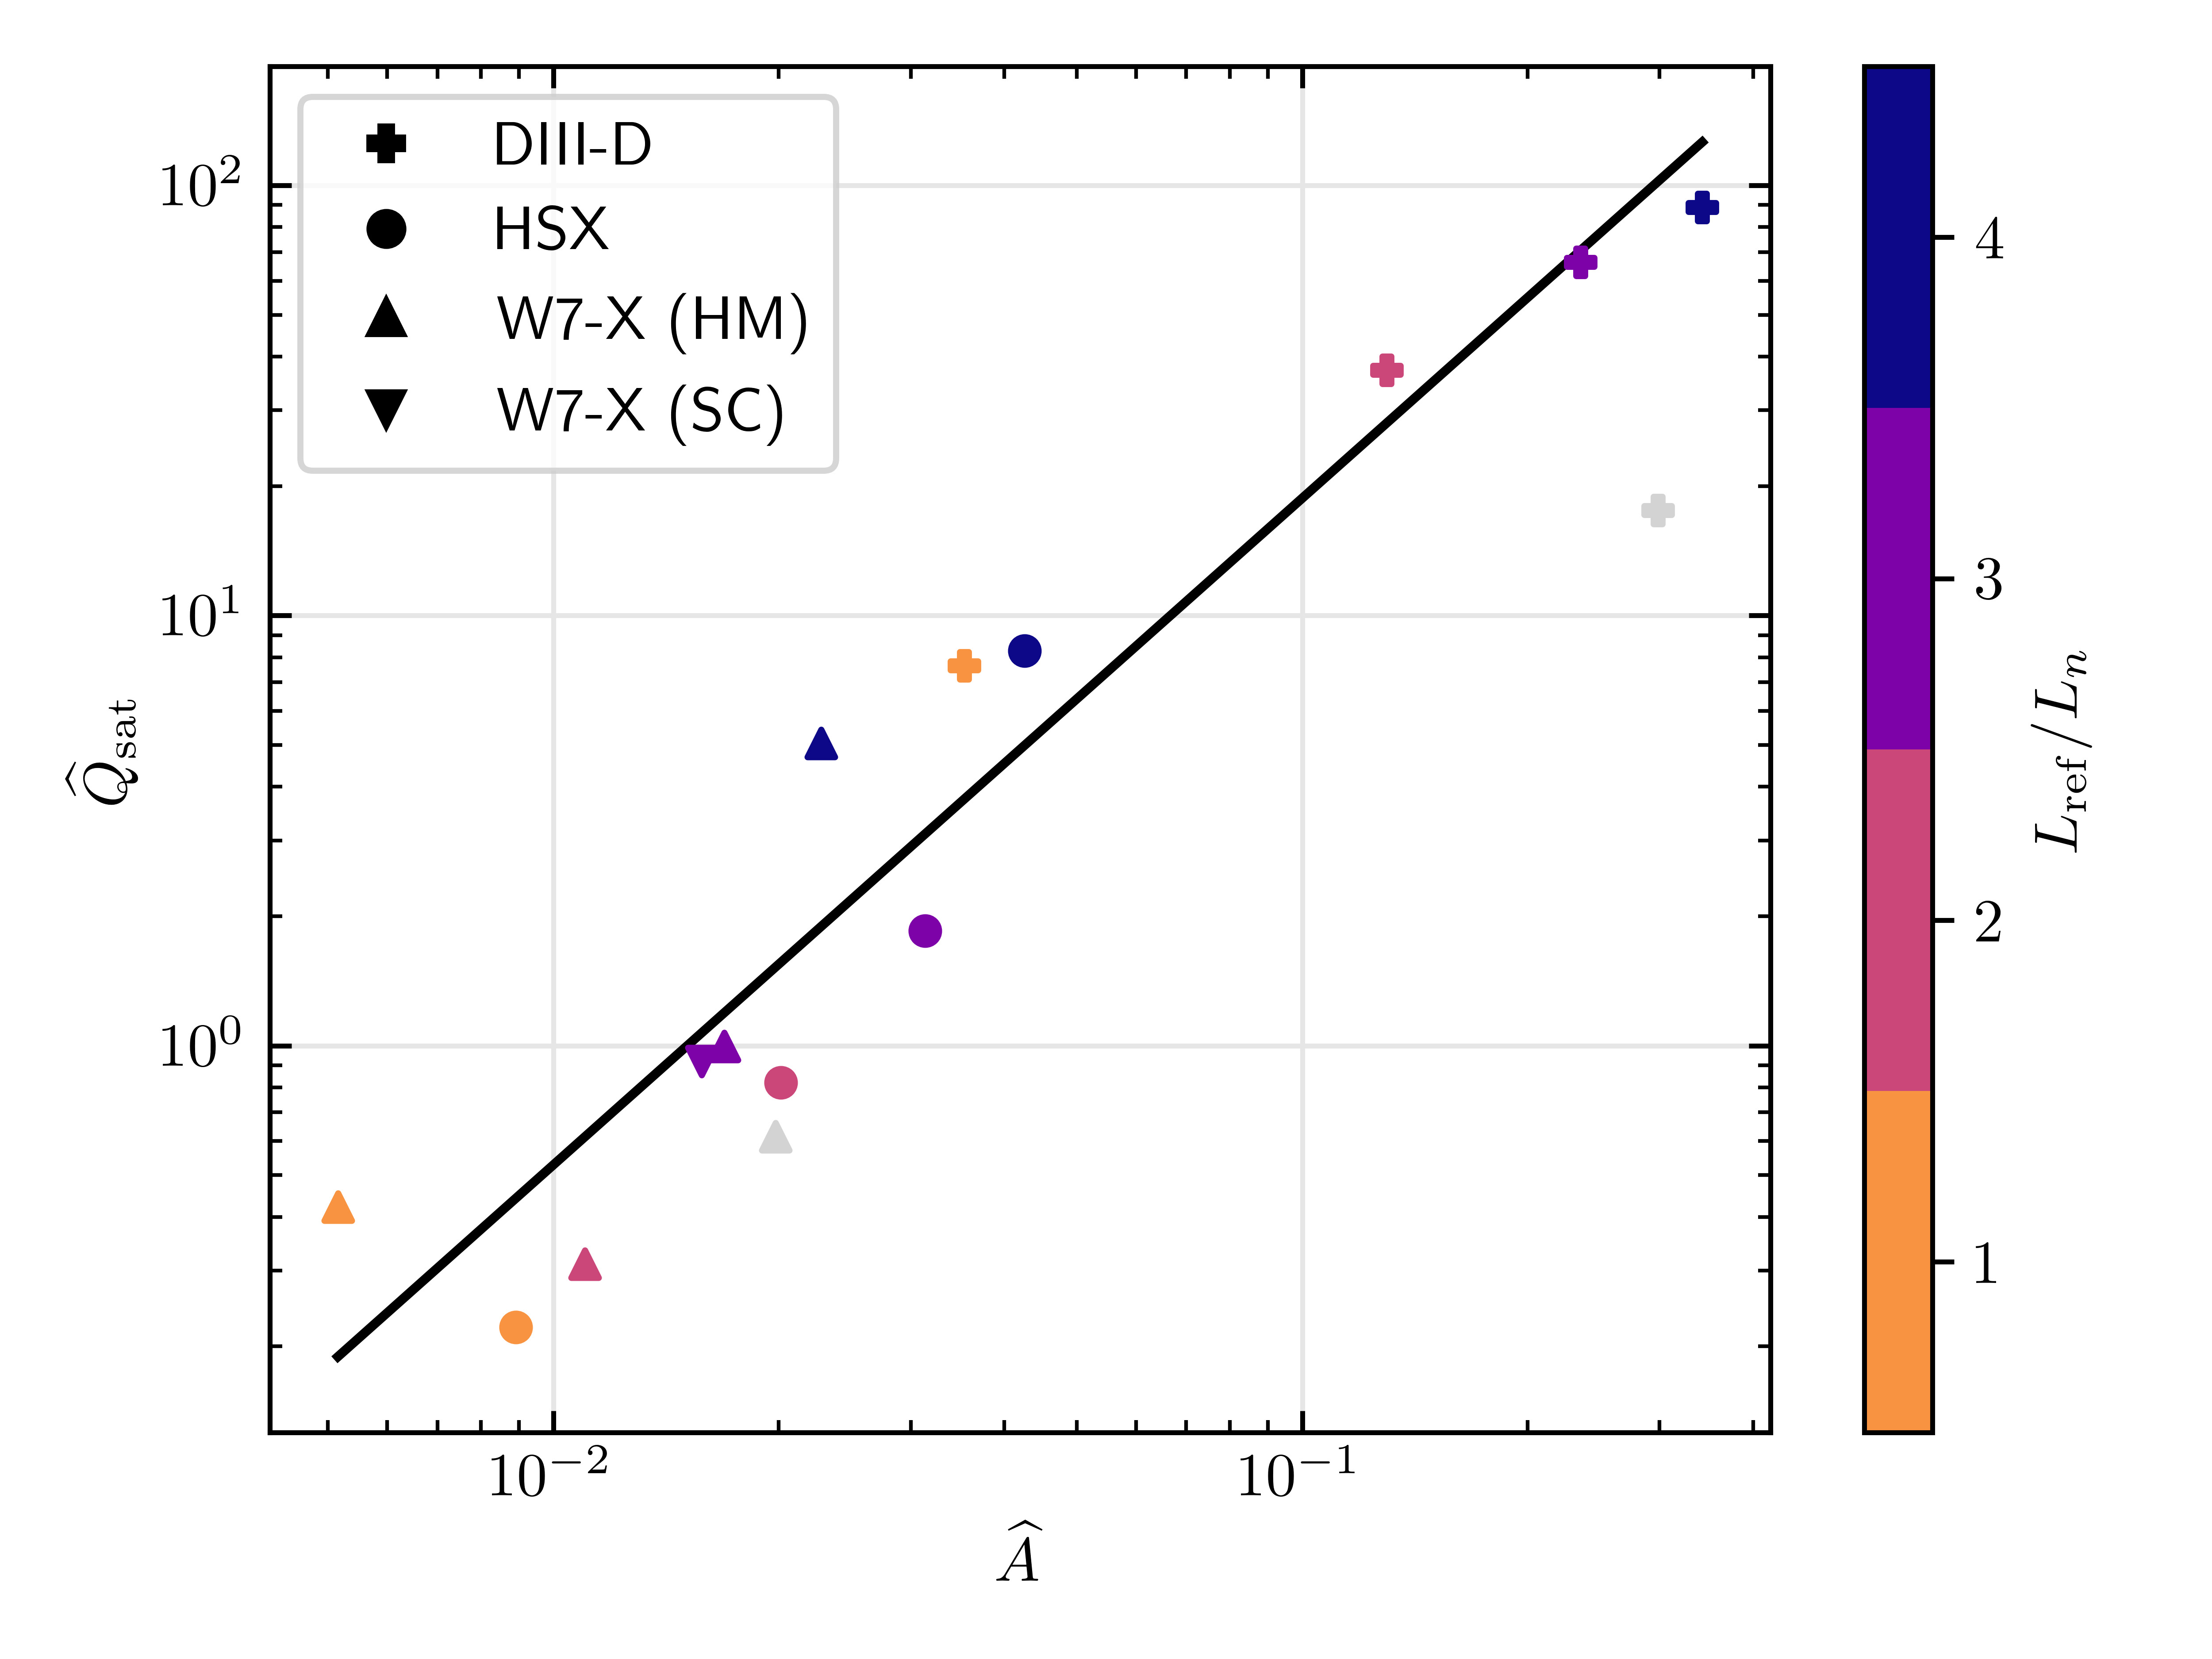
\includegraphics{3_chapters/1_papers/AE-TE/figures/plot_AE_Q_corr.png}
    \caption{A scatter plot showing the normalized \AE{} for a range of stellarator and tokamak plasmas and the average nonlinear saturated turbulent radial energy flux from gyrokinetic simulations of these plasmas. The different points refer to different density gradients, as indicated by the colour, and to different devices. The devices that are used in this analysis are the tokamak DIII-D, the Helically Symmetric eXperiment (HSX), and the W7-X stellarator in both high mirror configuration (HM) and standard configuration (SC). The straight black line shows the least-squares fit, which results in the power law $\ln Q_\text{sat} \propto (1.5 \pm 0.1) \ln A. $}
    \label{fig:scatter_plot_AE}
\end{figure}
A power law is found by fitting a straight line to the log-log plot given in Fig. \ref{fig:scatter_plot_AE}, where we have excluded the grey points from the fitting procedure. The fit results in
\begin{equation}
    Q_\text{sat} \propto A^{1.5 \pm 0.1}.
\end{equation}
This relation is of interest, as it can be motivated in the following manner. The electron energy flux density in the direction of $\nabla x$ is defined as
\begin{equation}
    \begin{aligned}
        {Q}_e &= \frac{1}{V_\text{sim}} \int \epsilon f_{e1} (\boldsymbol{v}_D \cdot 
        \rho\nabla x) \mathrm{d} \boldsymbol{x}.
    \end{aligned}
\end{equation}
Here, $\boldsymbol{v}_D$ is the gyro-averaged drift velocity, and $f_{e1}$ is the fluctuating part of the electron distribution function \citep{Gorler2010MultiscaleMicroturbulence}. We go on to crudely estimate this flux as
\begin{equation*}
    Q_e \sim \sqrt{\langle \mathbf{v}_D^2 \rangle} \int \epsilon f_{e1} \, \mathrm{d} \boldsymbol{x},
\end{equation*}
where the angular brackets denotes an average over the simulated volume.
The integral in this expression is bounded by the \AE{}, and hence we set $\int \epsilon f_{e1} \mathrm{d} \boldsymbol{x} \sim A$. The average of the squared drift velocity,
\begin{equation*}
    \langle \mathbf{v}_D^2 \rangle = \left\langle \left( \mathbf{E} \times \mathbf{B} / B^2 \right)^2 \right\rangle,
\end{equation*}
is proportional to the gyrokinetic energy of the electric field. Since the sum total of the thermal and this field energy should be conserved \cite{Helander2017AvailablePlasmas}, this field energy is also bounded by the \AE{}. We thus estimate that $\langle \mathbf{v}_E^2 \rangle \sim A$, which gives
\begin{equation}
    Q_e \propto A^{3/2},
\end{equation}
in agreement with the observed power-law. We have furthermore tried different conditions for particles which cross the computational boundary \citep{mackenbach2023bounceaveraged}, and we find that the results are resilient against these such variations. \par 
The two grey points lie significantly below the black line in Fig.~\ref{fig:scatter_plot_AE}. A possible reason may be that all the other points refer to plasmas with a density gradient, in which there is, in principle, \AE{} in both the electron and ion populations (although we have only considered the electons). In contrast, for the grey points correspond to plasmas with an electron gradient alone, implying that the \AE{} from the ions vanishes identically. There is thus less energy to drive turbulence in this case. 

\subsection{The distribution of \AE{}}
We now go on to investigate how different trapped particle orbits contribute to the \AE{}. In order to do so, we define an \AE{} per trapping well, namely
\begin{equation}
    \begin{aligned}
        \widehat{A}_\lambda(\lambda) = \int_0^\infty & e^{-z} z^{5/2}  \left[ \hat{\omega}_{\alpha}^2 \left( \frac{ \hat{\omega}_{*}^T }{\hat{\omega}_{\alpha}} - 1 +  \hat{F} \right) + \hat{\omega}_{\psi}^2 \left( -1 + \hat{F} \right)  \right] \hat{G}^{1/2} \mathrm{d}z,
    \end{aligned}
    \label{eq:ae-per-lam}
\end{equation}
so that $\int \sum_{\mathrm{wells}} \widehat{A}_\lambda \mathrm{d} \lambda = \widehat{A}$.
For any given value of $\lambda$, this quantity can be calculated separately for each trapping well. The  bounce points associated with each $\lambda$, which we denote by $\theta_b$ (with $\theta$ being the poloidal angle, our field-line following coordinate), satisfy 
\begin{equation}
    1 - \lambda \hat{B}(\theta_b) = 0.
    \label{eq:relation-lambda-bounce-points}
\end{equation}
One can then draw a straight line between the two bounce-points of a bounce-well, and one can color that line according to its associated $A_\lambda$. One can furthermore investigate $\hat{\omega}_\alpha$ and $\hat{\omega}_\psi$ as a function of their bounce points. This can be done by realising that both $\hat{\omega}_\alpha$ and $\hat{\omega}_\psi$ can be mapped onto their bounce points using equation \eqref{eq:relation-lambda-bounce-points}, and one can thus investigate how their values depend on the bounce-points.
\par 
A plot displaying the properties of equation \eqref{eq:ae-per-lam} in this way is shown in Fig. \ref{fig:AE_per_bw_D3D} for the case of the DIII-D tokamak with a normalised density gradient $L_\mathrm{ref}/L_n = 3$. Additionally, the binormal and radial drifts are shown as dashed green and dash-dotted blue lines, respectively. For convenience, a black dotted line is also displayed which indicates where $\hat{\omega}_\psi = \hat{\omega}_\alpha = 0$. It can be seen that energy is available over most of the magnetic well. Only the most shallowly trapped particles do not contribute to the \AE{}, as $\hat{\omega}_\alpha$ changes sign for these particles. This is in line with expectations, as the more deeply trapped particles experience ``bad curvature'' only, which in turn drives the TEM unstable \citep{Proll2012ResilienceInstabilities,Helander2017AvailablePlasmas}. The contribution to the \AE{} from the trapped particle orbits is enhanced by the positive magnetic shear in DIII-D \citep{connor1983effect}. The most shallowly trapped particles experience good curvature along most of their trajectories and exert, in contrast to the deeply trapped particles, a stabilising influence. Note that this figure refers to a tokamak, which besides being exactly omnigenous only has a single trapping well. Stellarators generally have many different bounce wells, and non-omnigenous effects arise due to net radial drifts.
\begin{figure}
    \centering
    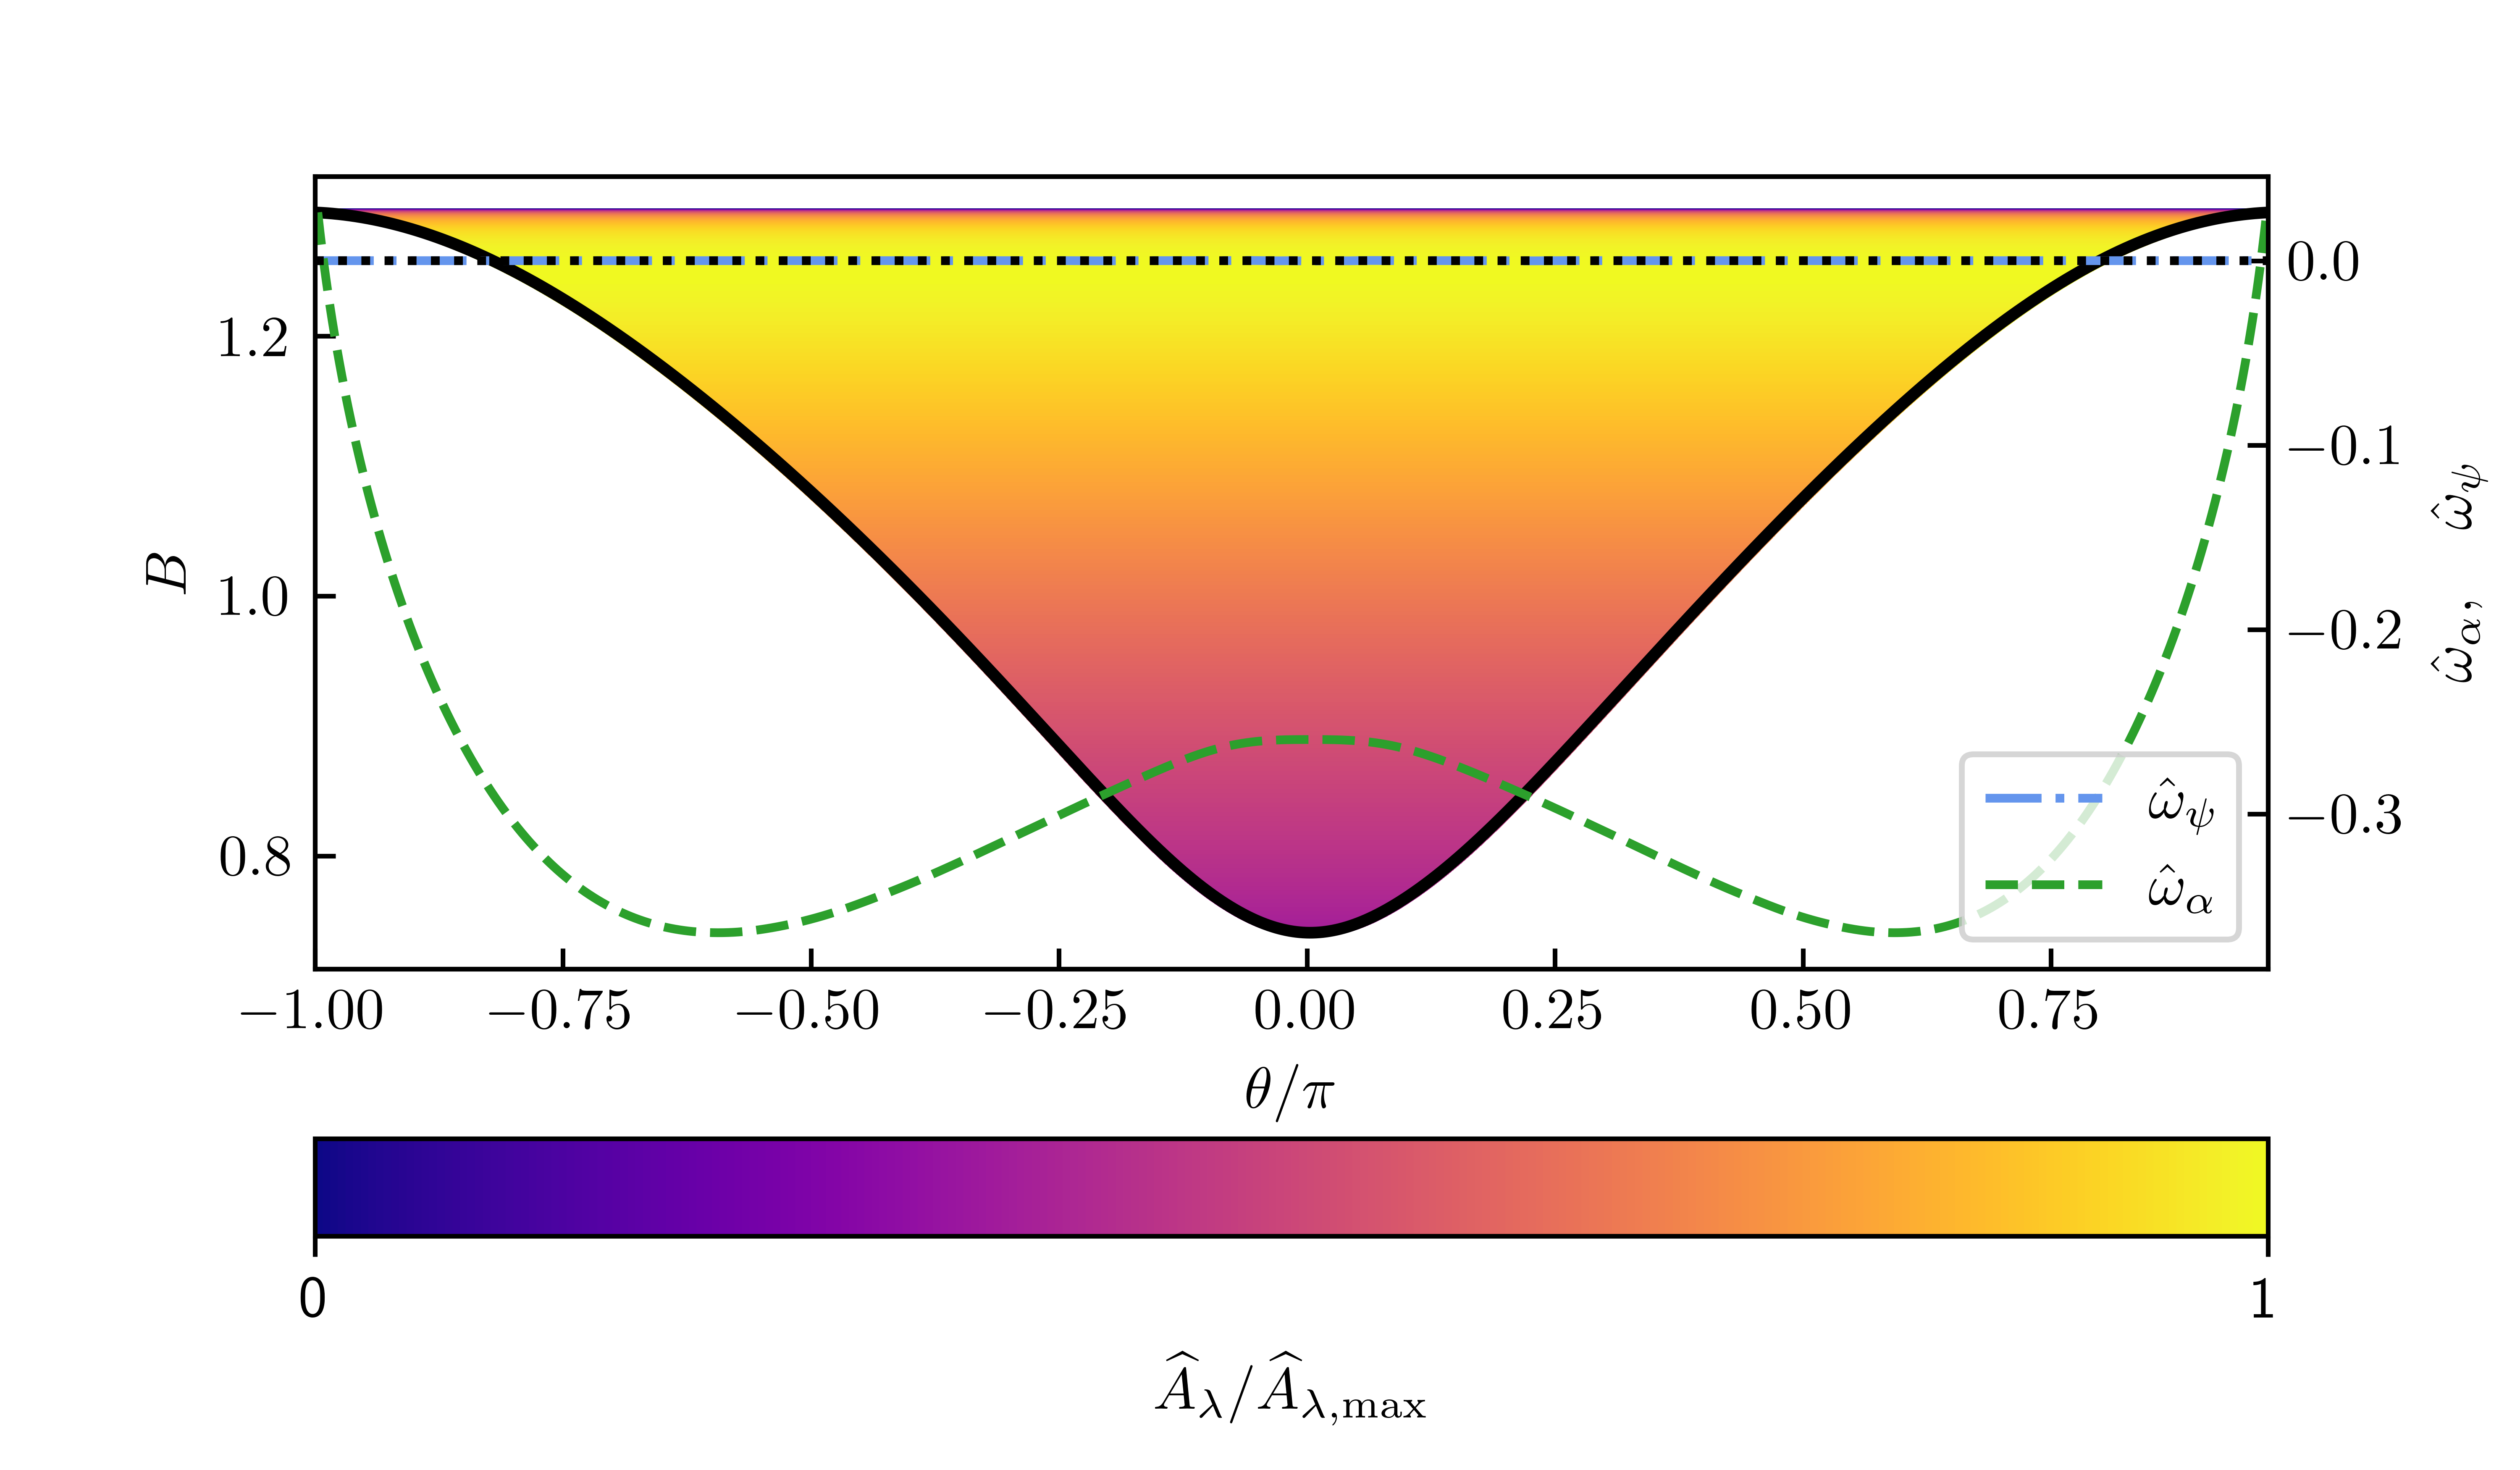
\includegraphics[width=\textwidth]{3_chapters/1_papers/AE-TE/figures/AE_per_lam_D3D.png}
    \caption{The \AE{} per $\lambda$ for DIII-D. The flux tube is located a normalized radial flux of $\psi/\psi_\mathrm{edge}=0.5$.}
    \label{fig:AE_per_bw_D3D}
\end{figure}
\par 
To investigate how these circumstances change the distribution of \AE{} across different bounce wells, we show a plot of W7-X in its standard magnetic configuration in Fig. \ref{fig:AE_per_bw_W7X}, with a density gradient of $L_\mathrm{ref}/L_n = 3$. Several interesting features can be seen. The most pronounced difference to the previous figure is that the \AE{} is much more localized than in DIII-D, so that most of the contribution comes from a narrow range of bounce wells. Most of the \AE{} comes from bright bands in the central well, particularly those where the bounce well approaches the local maximum in $B$ around $\theta = 0$. One can understand this observation in the following manner. Near the local maximum in field strength, the drift is maximally bad (as $\hat{\omega}_\alpha$ is most negative), and the trapped particles in this region contribute significantly to the \AE{}. Furthermore, the \AE{} is weighted by $\hat{G}^{1/2}$, which is proportional to the bounce time, which becomes large near such a local maximum. These two effects combine in the central region, giving rise to the large \AE{} there. One can also see two bright bands at $B \approx 1.10$, which at first seems puzzling as the particles experience average good curvature in this band as indicated by the positive sign of $\hat{\omega}_\alpha$. However, these particles experience a net radial drift ($\hat{\omega}_\psi \neq 0$) and this non-omnigenity causes the \AE{} to be non-zero. Furthermore, it is exacerbated by the large bounce time, resulting in the bright bands seen in the figure. Finally, one can see that, as in a tokamak, shallowly trapped particles barely contribute to the \AE{}, though the fraction of trapped particles which do not contribute is significantly larger than in DIII-D. \par
\begin{figure}
    \centering
    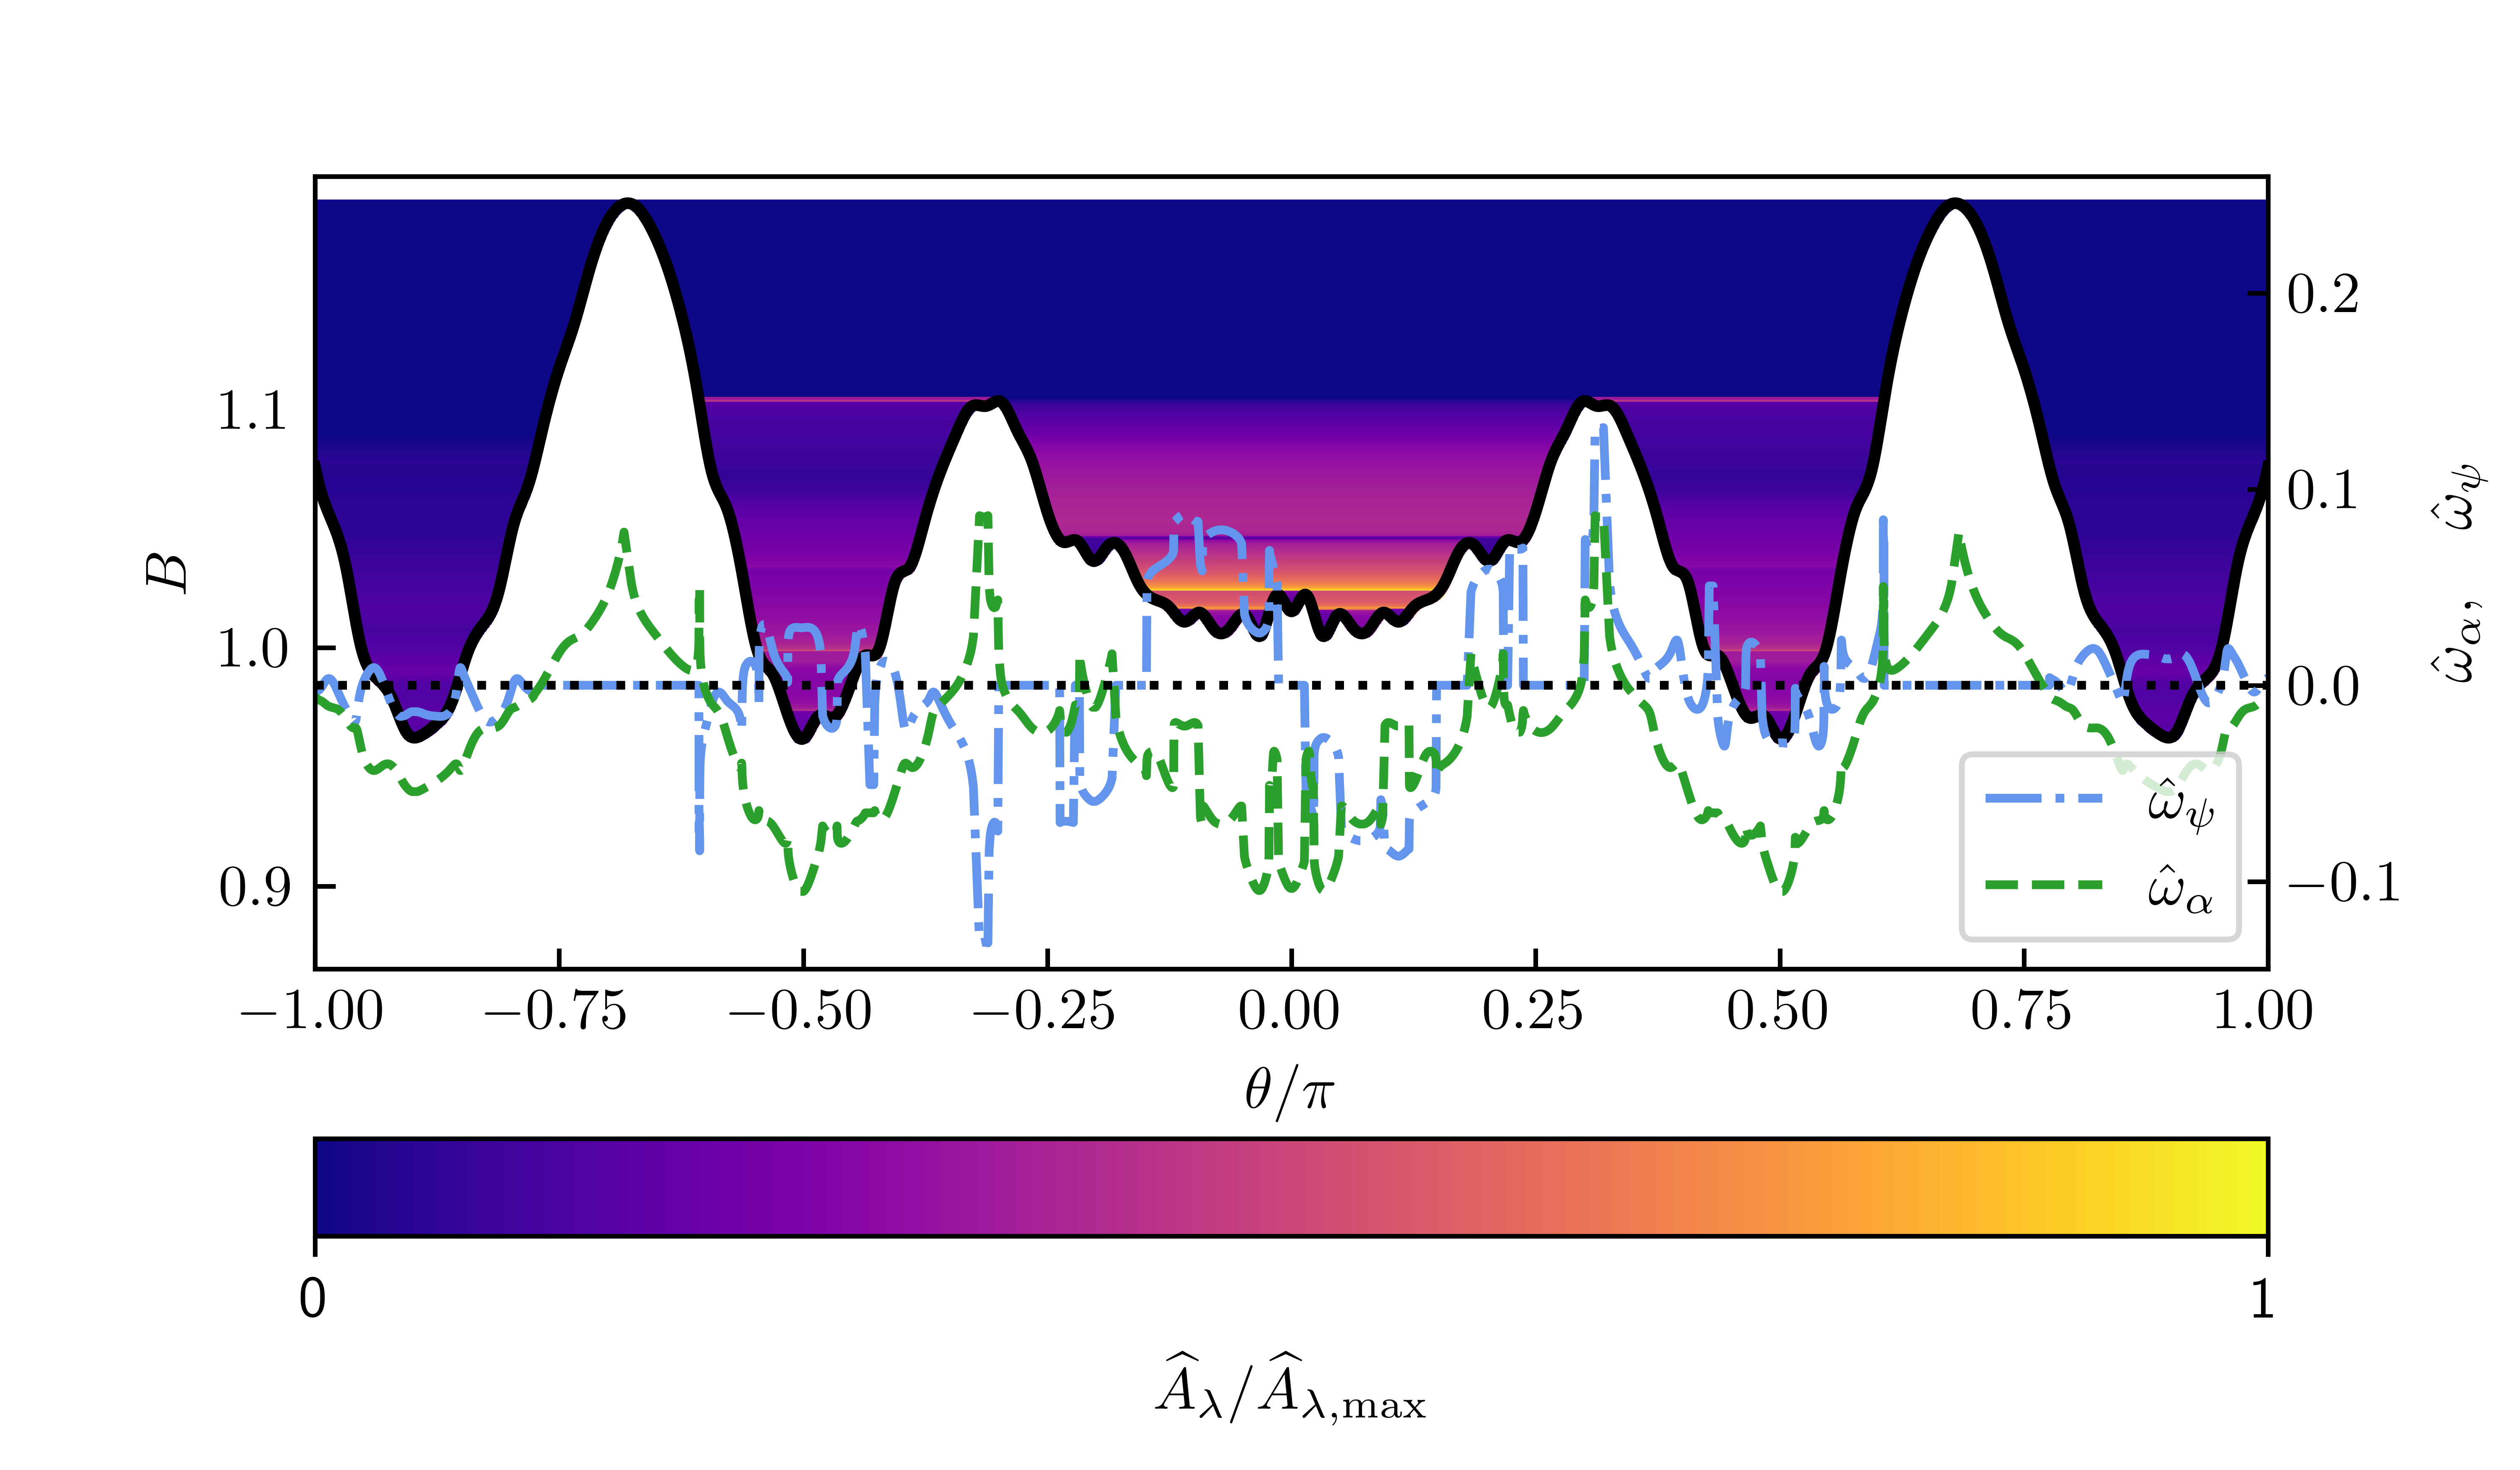
\includegraphics[width=\textwidth]{3_chapters/1_papers/AE-TE/figures/AE_per_lam_W7XSC.png}
    \caption{The \AE{} per $\lambda$ for W7-X (SC). The flux tube is located a normalized radial flux of $\psi/\psi_\mathrm{edge}=0.5$.}
    \label{fig:AE_per_bw_W7X}
\end{figure}
In summary, the distribution of \AE{} across various bounce wells indicates that it is the deeply trapped particles in regions of bad curvature which tend to be most destabilizing. Furthermore, the bounce-time plays an important role in determining which particles contribute most to the \AE{}. Finally, we note that non-omnigenous effects can destabilize otherwise stable regions.
\subsection{Dependence on gradient strength}
We finally investigate how the \AE{} depends on the strength of the gradient $\hat{\omega}_*^T$, when all other variables are kept constant. In the limit of large gradients, it is easy to see that equation \eqref{eq:normalized-AE-final} implies a linear scaling with the gradient strength. We go one step further and expand the integrand around large $\omega_*^T$, which gives
\begin{equation}
    \widehat{A} \propto  \hat{\omega}_*^T \left (\hat{\omega}_\alpha + \mathrm{sgn}(\hat{\omega}_*^T) \sqrt{\hat{\omega}_\alpha^2 + \hat{\omega}_\psi^2} \right) \hat{G}^{1/2},
\end{equation}
where $\mathrm{sgn}(x)=x/|x|$ is the sign function. In the opposite limit of small gradients, we find an important distinction between omnigenous and non-omnigenous devices. In a non-omnigenous device, one can expand equation \eqref{eq:AE-per-total-energy} around small $\hat{\omega}_*^T$, and one finds that in a weakly driven regime the integrand becomes
\begin{equation}
    \widehat{A} \propto (\hat{\omega}_*^T)^2 \frac{\hat{\omega}_\psi^2}{\hat{\omega}_\alpha^2+\hat{\omega}_\psi^2} \hat{G}^{1/2}
\end{equation}
For an exactly omnigenous device, however, this result vanishes due to the factor $\hat{\omega}_\psi^2$. To find the correct scaling for such devices, we return to the expression for the \AE{} of an omnigenous device first found in \cite{Helander2020AvailablePlasmas}. Here it was found that the \AE{} is proportional to
\begin{equation}
    \widehat{A} \propto \iint e^{-z} z^{5/2} \hat{\omega}_\alpha^2 R \left[ \frac{\hat{\omega}_*^T}{\hat{\omega}_\alpha} - 1 \right] \hat{G}^{1/2}  \mathrm{d} \lambda \mathrm{d} z,
\end{equation}
where $R[x] = (x + |x|)/2$ is the ramp function. Note that when $\hat{\omega}_*^T$ is small, the ramp function is non-zero in the region where $\omega_\alpha \rightarrow 0$. If we assume there exists a point where $\omega_\alpha=0$ we can expand around the point $\hat{\omega}_\alpha(\lambda_0) = 0$, and set
\begin{equation}
    \hat{\omega}_\alpha \approx \hat{\omega}_\lambda (\lambda - \lambda_0).
\end{equation}
Next we find the region where the argument of the ramp function is positive by finding where the argument vanishes,
\begin{equation}
    \frac{\hat{\omega}_*^T}{\hat{\omega}_\alpha} - 1 = 0 \implies \lambda \approx \lambda_0 +  \frac{\hat{\omega}_*^T}{\hat{\omega}_\lambda}.
\end{equation}
We can now perform the integral over the range $\lambda \in [\lambda_0,\lambda_0+ \hat{\omega}_*^T/\hat{\omega}_\lambda]$, and we find that the \AE{} to leading order is proportional to
\begin{equation}
    \widehat{A} \propto \int e^{-z} z^{5/2} \hat{\omega}_\lambda \hat{\omega}_*^T \left( \frac{\hat{\omega}_*^T}{\hat{\omega}_\lambda} \right)^2  \hat{G}^{1/2}(\lambda_0) \mathrm{d}z.
\end{equation}
Thus we conclude that, for weakly driven omnigenous devices, the \AE{} integrand scales as
\begin{equation}
    \widehat{A} \propto |\hat{\omega}_{*}^{T}|^3 \frac{\hat{G}^{1/2}(\lambda_0)}{|\hat{\omega}_\lambda|}.
\end{equation}
Hence in summary we have
\begin{equation}
\widehat{A} \propto
    \begin{cases}
        (\hat{\omega}_*^T) & \text{if } |\hat{\omega}_*^T| \gg 1 \\
        ( \hat{\omega}_*^T)^2 & \text{if } |\hat{\omega}_*^T| \ll 1 \text{ and } \hat{\omega}_\psi \neq 0 \\
        ( \hat{\omega}_*^T)^3 & \text{if } |\hat{\omega}_*^T| \ll 1 \text{ and } \hat{\omega}_\psi = 0
    \end{cases}
\end{equation}
\par 
\begin{figure}
    \centering
    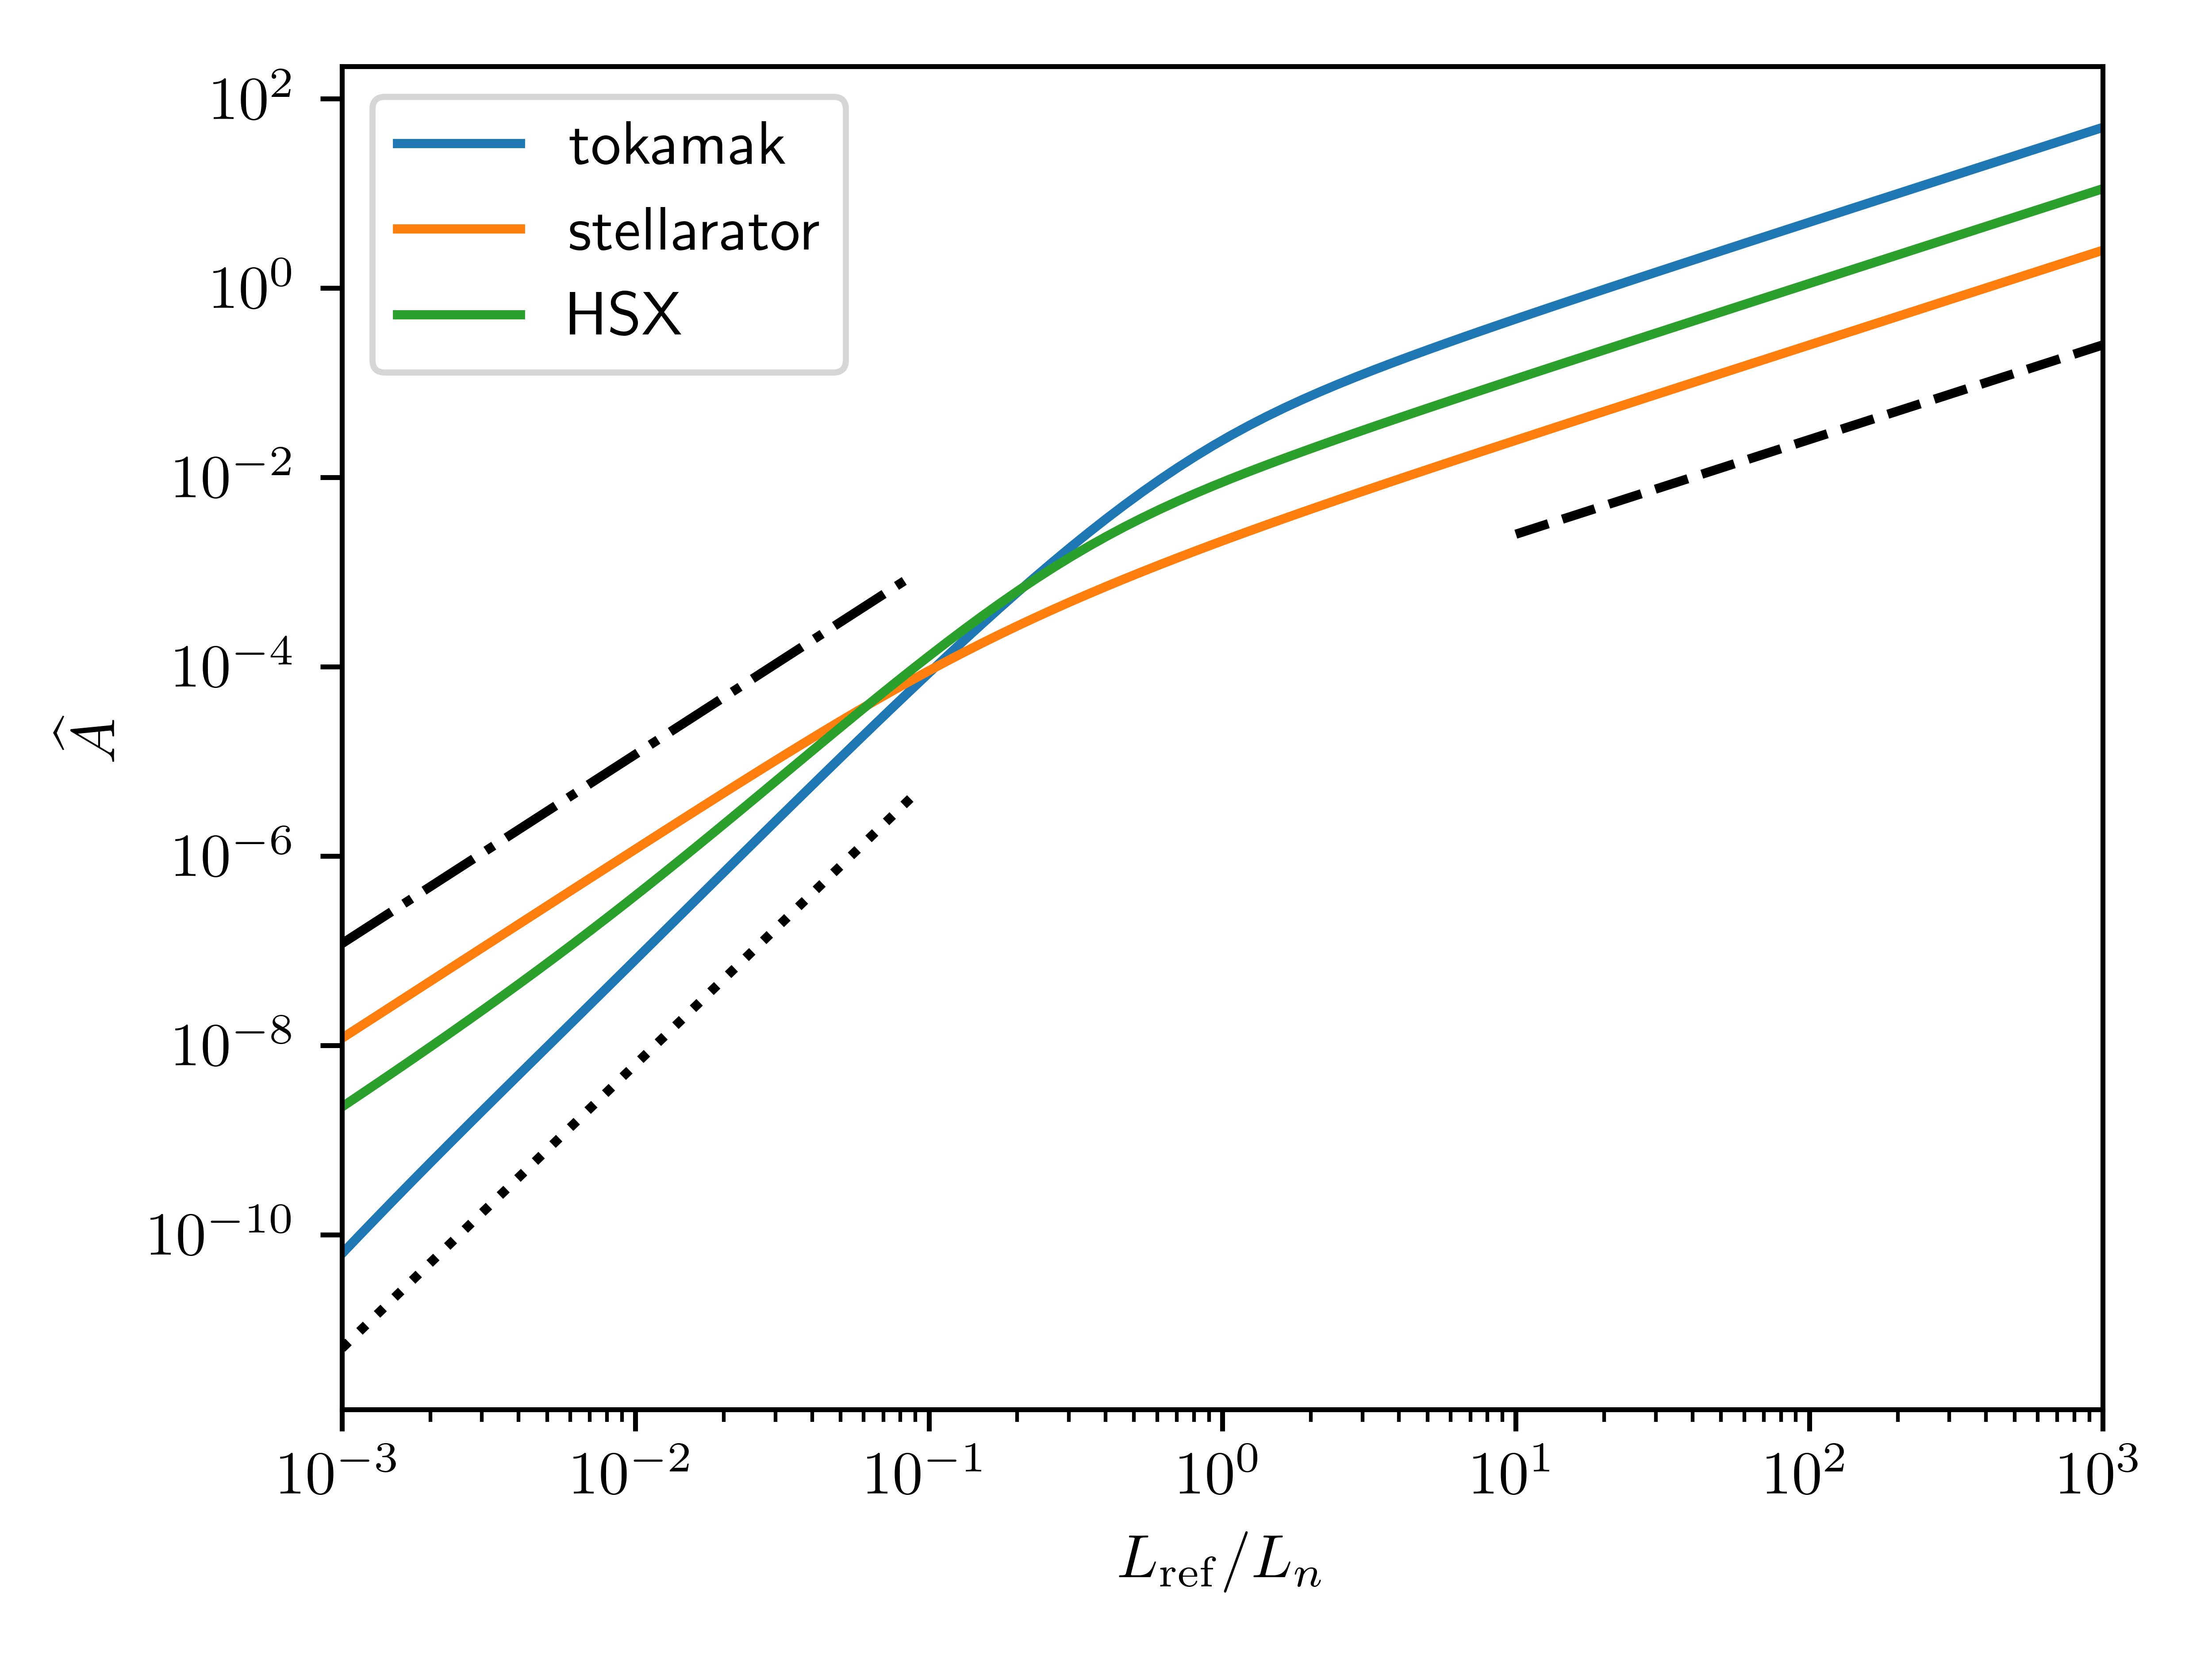
\includegraphics{3_chapters/1_papers/AE-TE/figures/gradient-scaling.png}
    \caption{An example of the dependence of \AE{} on the gradient strength for three different devices; a tokamak, a non-omnigenous stellarator, and HSX. In the case displayed above, the electron temperature gradient is set to zero. The dashed, dash-dotted, and dotted lines have a linear, square, and third power scaling with the density gradient, respectively}
\label{fig:scaling-laws}
\end{figure}
The different scaling laws are displayed in Fig. \ref{fig:scaling-laws}, where we see a tokamak (which is exactly omnigenous), a non-omnigenous stellarator, and the optimized, fairly omnigenous, HSX stellarator. The plots show a distinct ``knee'' at the transition from one scaling law to the next. This knee is especially pronounced for the tokamak, and less so for the stellarator. The difference in scaling for weakly and strongly driven regimes is interesting, as the behaviour is reminiscent of gradient-threshold (also called critical-gradient) type behaviour. Such a gradient-threshold is signified by small transport up to some threshold in the gradient followed by strong transport above this threshold \citep{Dimits2000ComparisonsSimulations}, a behaviour shared by the present plot. It is thought that this critical gradient plays an important role in profile stiffness, where profiles tend to retain their shape without much sensitivity to the details of the particle/energy sources \citep{garbet2004profile}. It is also interesting to note that, from the different scaling laws for omnigenous and non-omnigenous devices, one would expect the critical-gradient-like behaviour of the \AE{} to be ``softer'' in an non-omnigenous stellarator, as the transition from a quadratic to a linear scaling law is more gradual than that from a cubic one. If this gradient-threshold behaviour of the \AE{} indeed corresponds to the true critical gradient, this would result in profiles being less stiff, which has indeed observed in various stellarators \citep{milligen2008quantifying,sanchez2015self}. Investigating HSX more closely, we see that for very low gradients it follows a quadratic scaling, for moderate gradient it approaches a third-power scaling, and for strong gradient it is linear. This third-power region is a result of HSX being close to quasi-symmetry, so that $\hat{\omega}_\psi$ is small. However, at small enough gradients, the $\hat{\omega}_\psi$ term starts to become important causing the scaling to be quadratic. 
\par 
Finally, we note the non-trivial dependence on $\hat{\omega}_\alpha$ in the various regimes. When the gradients are large, the \AE{} is linearly proportional to $\hat{\omega}_\alpha$, which quantifies ``bad curvature'', but for small gradients it is {\em inversely} proportional to $\hat{\omega}_\alpha$. This implies that one can \emph{reduce} the total \AE{} by increasing the amount of bad curvature. This would lead to reduced \AE{} in the weakly driven regime, and the ``knee''-point would be shifted to higher $\hat{\omega}_*^T$, which would lead to a higher critical gradient (as estimated from \AE{}). This is in line with recent results of \cite{roberg2022coarse,roberg2023critical}, who found that the critical gradient can be increased by introducing more bad curvature into the magnetic geometry, which thus leads to  lower turbulent heat-fluxes, though it should be noted that those results concern ion-temperature gradient driven transport. An important corollary of this property is that, in a device with particularly low \AE{} in the weakly-driven regime (much bad curvature), the \AE{} becomes very large in the strongly-driven regime, being linearly proportional to $\hat{\omega}_\alpha$ when $\hat{\omega}_*^T \gg 1$. One can thus either have a device with a high gradient-threshold and low \AE{} for small gradients (which may be attained by increasing the amount of bad curvature), or a device with low \AE{} in the strongly driven regime thanks to relatively little bad curvature in regions with many trapped particles.

\section{Summary and conclusions} 
\label{sec:conclusions}
In this paper we have derived the \AE{} of trapped electrons in a slender flux-tube of magnetically confined plasma, and we have compared it with nonlinear saturated radial electron energy fluxes as calculated by nonlinear gyrokinetic simulations. In deriving the \AE{}, several key insights were required to make progress. Firstly, it was found that the calculation is particularly simple in flux tubes with elliptical cross section. An explicit expression of the ground state can then be found, which was used to calculate the \AE{} to leading order. The result is positive definite, as it must be, and reduces to a previously found expression in the case that the magnetic field is omnigenous. Since the \AE{} depends on the cross section of the flux tube, its major and minor radii need to be chosen a priori. The correct choice depends on the correlation length of the turbulence, which we take to be proportional to the gyroradius in both directions.
\par
We compared the resulting \AE{} for different magnetic geometries with the energy flux computed in a set of simulations of density-gradient driven turbulence. The numerical \AE{} calculations are many orders of magnitude faster than the gyrokinetic simulations. The analysis is done for 4 different magnetic configurations, DIII-D, HSX, and W7-X in its standard and high mirror configurations. The saturated electron energy flux $Q_\text{sat}$ is approximately related to the \AE{} via a simple power law $Q_\text{sat} \propto A^{1.5 \pm 0.1}$. A straightforward phenomenological model to explain the observed power law is proposed, which results in $Q_\text{sat} \propto A^{3/2}$. We go on to investigate which regions are driving the available energy. The results can be understood in terms of simple geometrical concepts: bad curvature (resulting in the drift being in resonance with the drift wave) and non-ommigenity drive \AE{}. We finally investigate the dependence of \AE{} on gradient and find that there are three distinct scaling laws; for strong gradients the \AE{} scales linearly with the gradient strength, whereas for weak gradients the \AE{} scales as the gradient-strength squared or cubed for non-omnigenous or exactly onigenous fields, respectively. 
\par 
These results are interesting for future research. The strong correlation between \AE{} and energy flux across various devices indicates that it may serve as a good proxy-function for stellarator optimisation codes\citep{Spong2001PhysicsStellarators,landreman2021simsopt} used to design stellarators with reduced turbulence. Direct gyrokinetic simulations can be too time-consuming to be carried out inside the optimisation loop in such codes, so there is a need for more efficiently estimating turbulent transport in given magnetic field. It is thus of interest to understand how \AE{} is related to specific details in the field-line geometry. As we have seen, regions of bad curvature are associated with large \AE{}, thus providing a connection between previously known results from linear gyrokinetic stability theory and \AE{}, but the latter also seems to possess predictive qualities for nonlinear transport. Furthermore, one could also use the \AE{} derived here as a profile optimisation tool for TEM-dominated devices. One could then search for plasma profiles and adjustable coil currents which minimize the \AE{}, under some set of constraints. Finally, it may also be valuable to extract expressions for \AE{} in more generic scenarios where turbulence is driven by an ion temperature gradients
\section*{Acknowledgements} \label{sec:acknowledgements}
The authors are grateful for the valuable discussions with, J.M. Duff, J. Ball, T. G\"orler, M.J. Pueschel, P. Mulholland, P. Costello, M.J. Gerard, and E. Rodriguez. This work was partly supported by a grant from the Simons Foundation (560651, PH), and this publication is part of the project ``Shaping turbulence – building a framework for turbulence optimisation of fusion reactors'', with Project No. \texttt{OCENW.KLEIN.013} of the research program ``NWO Open Competition Domain Science'' which is financed by the Dutch Research Council (NWO). This work has been carried out within the framework of the EUROfusion Consortium, funded by the European Union via the Euratom Research and Training Program (Grant Agreement No. 101052200 — EUROfusion). Views and opinions expressed are however those of the author(s) only and do not necessarily reflect those of the European Union or the European Commission. Neither the European Union nor the European Commission can be held responsible for them. 

\renewcommand\thesection{\Alph{section}}
\setcounter{section}{0}

\section{Details of the derivation of the domain shape} \label{app:diff-for-domain}
Here we provide mathematical details for the argument given in Section \ref{sec:theory} concerning the domain shape. 
We do so by means of a geometric argument, sketched in Fig. \ref{fig:proof-of-domain-sketch}. Here $\mathrm{A}$ and $\mathrm{A}'$ denote two points on the boundary with parallel tangents, $T_{\mathrm{A}}$ and $T_{\mathrm{{A}'}}$, respectively. The distance between these tangents is $2D$ and the radius of curvature of the boundary at $\mathrm{A}$ is $R$. If $\mathrm{C}$ is the point on $T_{\mathrm{A}'}$ that is closest to $\mathrm{A}$ we thus have $|\mathrm{AC}|=2D$. Next, we let $\mathrm{B}$ and $\mathrm{B}'$ denote boundary points in the vicinity $\mathrm{A}$ and $\mathrm{A}'$, respectively, such that the tangents through $\mathrm{B}$ and $\mathrm{B}'$ are parallel, and we denote by $\mathrm{E}$ the point on the tangent through $\mathrm{B}'$ that is closest to $\mathrm{B}$. Let us write the distance $|\mathrm{BE}|=2(D+\mathrm{d}D)$ and define $|\mathrm{A}'\mathrm{C}|=2L$. To leading order in smallness of $\mathrm{d} \vartheta$ we have $|\mathrm{DC}|=2D \mathrm{d} \vartheta$. Furthermore, to leading order $|\mathrm{B}'\mathrm{E}|=2L$, implying that $|\mathrm{FE}|=2L\mathrm{d}\vartheta$, where $\mathrm{F}$ denotes the intersection of $\mathrm{BE}$ and $\mathrm{A}'\mathrm{C}$. All in all we find the leading-order relations,
\begin{equation*}
\begin{aligned}
    |\mathrm{BE}|&=|\mathrm{AD}|+|\mathrm{FE}| \\
    2(D+ \mathrm{d}D) &= 2D + 2L \mathrm{d} \vartheta \\
    \frac{\mathrm{d}D}{\mathrm{d}\vartheta} &= L.
\end{aligned}
\end{equation*}
Next we investigate how $L$ changes under some small change $\mathrm{d}\vartheta$. Let us define $|\mathrm{B}'\mathrm{E}|=2L' = 2(L+ \mathrm{d}L)$. Since $|\mathrm{AB}|=|\mathrm{A}'\mathrm{B}'|=R\mathrm{d}\vartheta$ and $|\mathrm{CD}|=2D\mathrm{d}\vartheta$, we have
\begin{equation*}
\begin{aligned}
    2L'&= 2L + 2 R \mathrm{d} \vartheta - 2D\mathrm{d}\vartheta \\
    \frac{\mathrm{d}L}{\mathrm{d}\vartheta} &= R - D.
\end{aligned}
\end{equation*}
Combining these relations, one finds
\begin{equation}
    \frac{\mathrm{d}^2 D}{\mathrm{d} \vartheta^2} = R - D,
\end{equation}
\begin{figure}
    \centering
    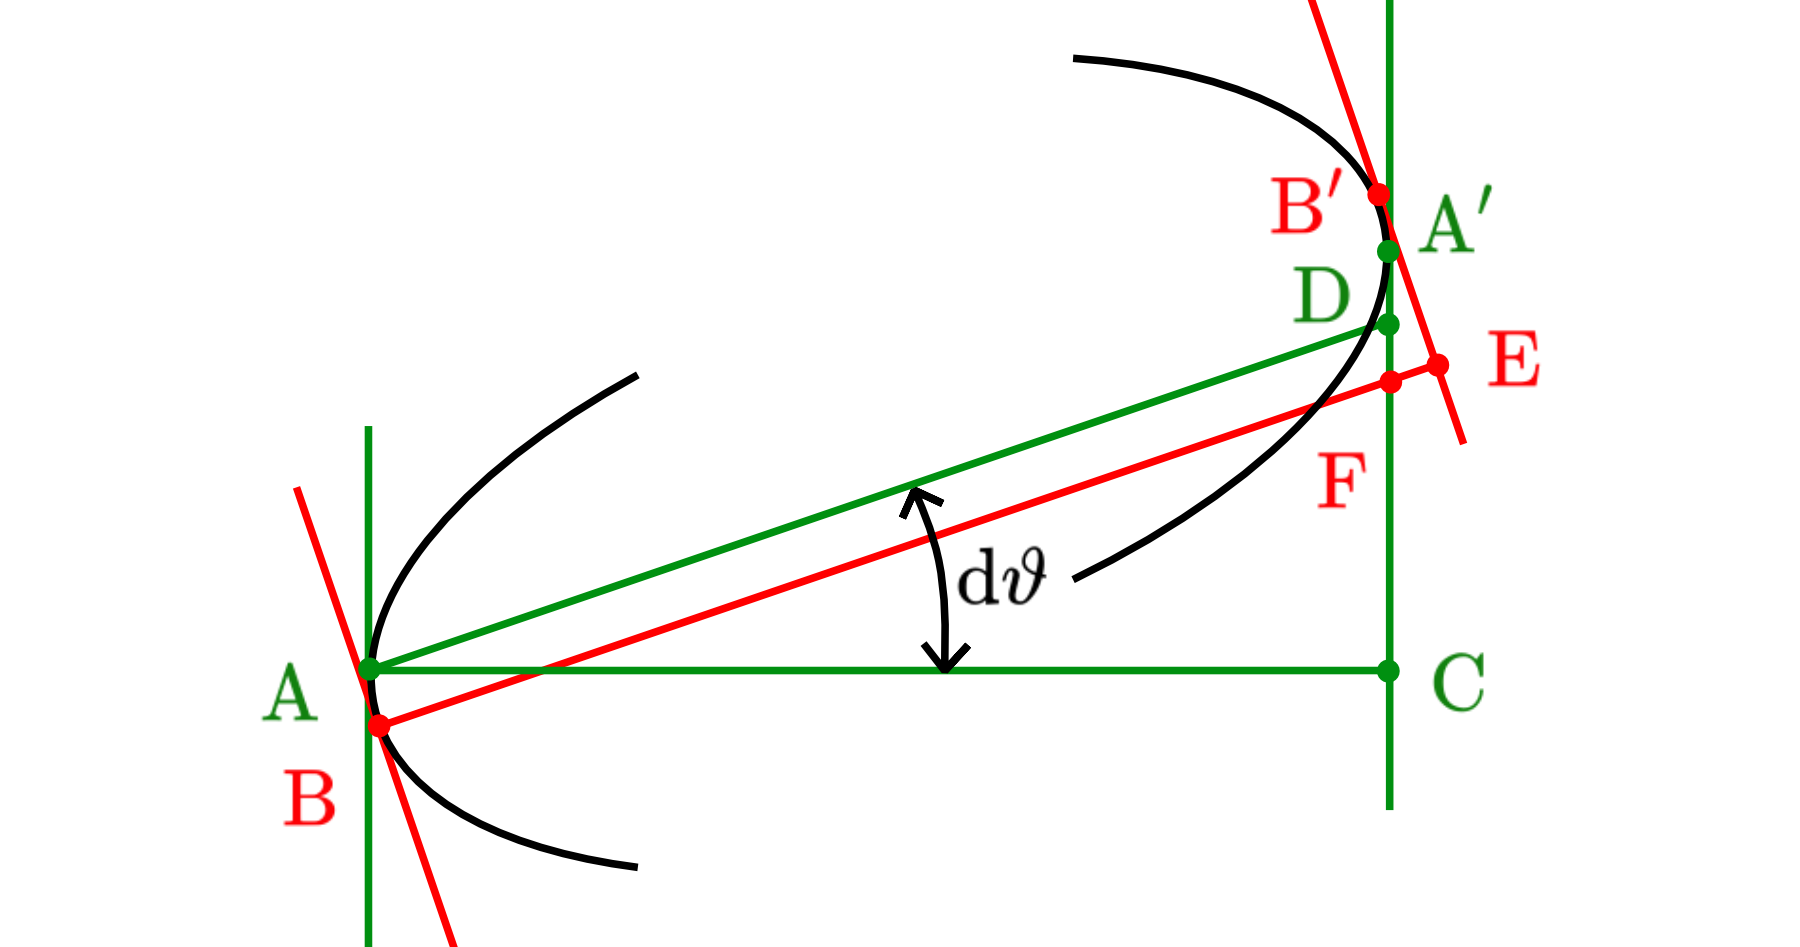
\includegraphics[width=0.8\textwidth]{3_chapters/1_papers/AE-TE/figures/boundary-proof-ellipse.png}
    \caption{A geometric sketch showing the relation between $D$ and $R$. The green vertical lines passing through $A$ and $A'$ are tangent to the boundary, as are the red ones passing through $B$ and $B'$.}
    \label{fig:proof-of-domain-sketch}
\end{figure}
and since $R = C_\mathcal{A}/D^3$ the equation for the domain can be written as
\begin{equation}
    \frac{\mathrm{d} D}{\mathrm{d} \vartheta} = \pm \sqrt{2C - D^2 - \frac{C_\mathcal{A}}{D^2}}.
\end{equation}
It is straightforward to solve for the inverse function, $\vartheta(D)$, which becomes
\begin{equation}
    \vartheta = \int \frac{\mathrm{d}D}{\sqrt{2C-D^2-\frac{C_\mathcal{A}}{D^2}}}
     = \frac{1}{2}\arcsin \left( \frac{D^2 - C}{\sqrt{C^2 - C_\mathcal{A}}} \right) + \mathrm{const.},
\end{equation}
where the integration constant constitutes an unimportant phase, which we can chosen conveniently, e.g., 
\begin{equation}
    D^2 = \sqrt{C^2-C_\mathcal{A}} (C  +\cos 2\vartheta)
\end{equation}
The radius of curvature thus becomes
\begin{equation}
    R(\vartheta) = \frac{C_\mathcal{A}}{(C^2-C_\mathcal{A})^{3/4}(C + \cos 2 \vartheta)^{3/2}}.
    \label{eq:radius-of-curv}
\end{equation}
Our final step is to verify that an ellipse has similar curvature. We first realise that
\begin{equation}
    \tan \vartheta = \frac{\mathrm{d} y}{\mathrm{d}x},
\end{equation}
which for an ellipse, $x^2/a^2 + y^2/b^2 = 1$ implies that 
\begin{equation}
    \tan \vartheta = - \frac{x}{y} \frac{b^2}{a^2}.
\end{equation}
Now, the radius of curvature for an ellipse may be written as
\begin{equation}
\begin{aligned}
    R &= (ab)^2 \left( \frac{\frac{x^2}{a^4} + \frac{y^2}{b^4}}{\frac{x^2}{a^2} + \frac{y^2}{b^2}} \right)^{3/2} \\
    &= \frac{b^2}{a} \left( \frac{1 + \frac{1}{\tan^2 \vartheta}}{1 + \frac{b^2}{a^2\tan^2 \vartheta}} \right)^{3/2} \\
    &=\frac{b^2}{a} \left( \frac{1}{1 + \frac{b^2/a^2-1}{2} (1 + \cos 2 \vartheta )} \right)^{3/2}.
\end{aligned}
\end{equation}
This is of the same form as Eq. \eqref{eq:radius-of-curv}, showing us that the ellipse is indeed the only sufficiently smooth solution to the problem.

\section{Relating derivatives to bounce-averaged frequencies}
\label{sec:appendix-bounce-freq}
Here we show how the derivatives of the energy and distribution function can be related to bounce averaged frequencies. By investigating the bounce-averaged Lagrangian of charged particles in electromagnetic fields, one can derive the following relations \citep{Helander2005CollisionalPlasmas,Helander2014TheoryFields},
\begin{equation}
    \frac{\partial \mathcal{J}}{\partial \alpha} = + q ( \delta \psi ), \qquad \frac{\partial \mathcal{J}}{\partial \psi} = - q ( \delta \alpha), \qquad \frac{\partial \mathcal{J}}{\partial \epsilon} = \tau_b.
\end{equation}
Here $\delta \psi$ is the total excursion in the $\psi$ direction after a full bounce motion, $\delta \alpha$ is the total excursion in the $\alpha$ direction after a full bounce motion, and $\tau_b$ is the bounce time. In general, we know that the second adiabatic invariant can be written as
\begin{equation}
    \mathcal{J} = \mathcal{J}(\epsilon,\psi,\alpha,\mu).
\end{equation}
Taking the total differential of $\mathcal{J}$ we thus find
\begin{equation}
    \begin{aligned}
        \mathrm{d}\mathcal{J}  = \tau_b \mathrm{d}\epsilon - q ( \delta \alpha ) \mathrm{d}\psi + q ( \delta \psi ) \mathrm{d}\alpha + \frac{\partial \mathcal{J}}{\partial \mu} \mathrm{d}\mu.
    \end{aligned}
\end{equation}
This allows us to readily find the derivatives of the energy function. We conclude that
\begin{subeqnarray}
    \left( \frac{\partial \epsilon}{\partial \psi} \right)_{\mu,\mathcal{J},\alpha} &&= + q \frac{\delta \alpha}{\tau_b} \equiv +  q\omega_\alpha, \\
    \left( \frac{\partial \epsilon}{\partial \alpha} \right)_{\mu,\mathcal{J},\psi} &&= - q \frac{\delta \psi}{\tau_b} \equiv - q \omega_\psi.
\end{subeqnarray}
With these findings the derivatives of the Maxwellian can readily be evaluated,
\begin{subeqnarray}
    \left(\frac{\partial f_{M}}{\partial \psi}\right)_{\mu,\mathcal{J},\alpha} &&= + q \frac{f_{M,0}}{T_0} \left( \omega_*^T - \omega_\alpha \right), \\
    \left(\frac{\partial f_{M}}{\partial \alpha}\right)_{\mu,\mathcal{J},\psi} &&= + q \frac{f_{M,0}}{T_0} \omega_\psi.
\end{subeqnarray}
Here, we have defined the electron diamagnetic drift frequency as $\omega_*^T$ as
\begin{equation}
    \omega_*^T \equiv \frac{T_0}{q} \frac{\mathrm{d} \ln n}{\mathrm{d} \psi} \left( 1 + \eta \left[ \frac{\epsilon_0}{T_0} - \frac{3}{2} \right] \right),
\end{equation}
and we have denoted the ratio between the gradients as $\eta = (\mathrm{d} \ln{T} / \mathrm{d} \psi ) / (\mathrm{d} \ln{n} / \mathrm{d} \psi )$.




% \section{The Jacobian of the phase-space reparameterisation}
%  \label{sec:appendix-phasespace-jac}
% Here we derive the Jacobian as we change phase-space variables,
% \begin{equation}
%     \mathrm{d}\boldsymbol{x} = \sqrt{g} \mathrm{d}\psi \mathrm{d}\alpha \mathrm{d}\mu \mathrm{d}\mathcal{J}.
% \end{equation}
% To make matters more convenient, we first calculate the Jacobian for the following transform,
% \begin{equation}
%     \mathrm{d}\boldsymbol{v} = \sqrt{g} \mathrm{d} \mu \mathrm{d}\epsilon.
% \end{equation}
% Firstly note that one can rewrite $\mathrm{d}\boldsymbol{v}$ in the following manner,
% \begin{equation}
%     \mathrm{d}\boldsymbol{v} = \frac{1}{2} \mathrm{d}(v_\perp^2)\mathrm{d}v_\parallel \mathrm{d}\zeta.
% \end{equation}
% Here, $v_\perp$ is the velocity perpendicular to the magnetic field line, $v_\parallel$ is the velocity parallel to the magnetic field line, and $\zeta$ is the gyration angle. We assume our system is independent of the gyration angle (i.e. we can integrate this angle out). We now realize that we can relate the remaining velocity coordinates to our new coordinates in the following manner,
% \refstepcounter{equation}
% \[
%     \mu = \frac{m v_\perp^2}{2 B}, \quad \epsilon = \mu B + \frac{1}{2}mv_\parallel^2. \eqno{(\theequation{\mathit{a},\mathit{b}})}
% \]
% Thus we find that the velocity-space volume element becomes
% \begin{equation}
%     \mathrm{d}\boldsymbol{v} = \frac{B}{\sqrt{\upi}} \left(\frac{2 \upi}{m}\right)^{3/2} \frac{\mathrm{d}\epsilon \mathrm{d}\mu}{ \sqrt{\epsilon - \mu B}}.
% \end{equation}
% We now focus on the real-space part of the transform, $\mathrm{d} \boldsymbol{r}$. We wish to express this real-space part in terms of Clebsch coordinates. We realize that the volume element changes as
% \begin{equation}
%     \mathrm{d} \boldsymbol{r} = \left[(\nabla \psi \times \nabla \alpha) \cdot \nabla \ell \right]^{-1} \mathrm{d} \psi \mathrm{d} \alpha \mathrm{d} \ell.
% \end{equation}
% Now, the magnetic field can be expressed in Clebsch coordinates in the following fashion \citep{Dhaeseleer2012FluxTheory},
% \begin{equation}
%     \boldsymbol{B} = \nabla \psi \times \nabla \alpha = B \frac{\partial \boldsymbol{r}}{\partial \ell}.
% \end{equation}
% Taking the inner product of the above equation with $\nabla \ell$, we thus find
% \begin{equation}
%     (\nabla \psi \times \nabla \alpha) \cdot \nabla \ell = B.
% \end{equation}
% Hence, the total phase-space volume element changes as
% \begin{equation}
%     \mathrm{d}\boldsymbol{x} = \frac{4 \upi}{m^2} \frac{\mathrm{d}\ell}{|v_\parallel|} \mathrm{d}\mu \mathrm{d}\epsilon \mathrm{d}\psi \mathrm{d}\alpha.
% \end{equation}
% We integrate over a bounce motion, giving
% \begin{equation}
%     \mathrm{d}\boldsymbol{x} = \frac{4 \upi}{m^2} \tau_b \mathrm{d}\mu \mathrm{d}\epsilon \mathrm{d}\psi \mathrm{d}\alpha.
% \end{equation}
% Finally, we replace the $\epsilon$ coordinate in favor of $\mathcal{J}$. This gives our final expression for the Jacobian,
% \begin{equation}
%     \mathrm{d}\boldsymbol{x} = \frac{4 \upi}{m^2} \mathrm{d}\mu \mathrm{d}\mathcal{J}  \mathrm{d}\psi \mathrm{d}\alpha.
% \end{equation}


\section*{Competing interests}
The authors declare no competing interests.